% Options for packages loaded elsewhere
\PassOptionsToPackage{unicode}{hyperref}
\PassOptionsToPackage{hyphens}{url}
\PassOptionsToPackage{dvipsnames,svgnames,x11names}{xcolor}
%
\documentclass[
  letterpaper,
]{krantz}

\usepackage{amsmath,amssymb}
\usepackage{iftex}
\ifPDFTeX
  \usepackage[T1]{fontenc}
  \usepackage[utf8]{inputenc}
  \usepackage{textcomp} % provide euro and other symbols
\else % if luatex or xetex
  \usepackage{unicode-math}
  \defaultfontfeatures{Scale=MatchLowercase}
  \defaultfontfeatures[\rmfamily]{Ligatures=TeX,Scale=1}
\fi
\usepackage{lmodern}
\ifPDFTeX\else  
    % xetex/luatex font selection
\fi
% Use upquote if available, for straight quotes in verbatim environments
\IfFileExists{upquote.sty}{\usepackage{upquote}}{}
\IfFileExists{microtype.sty}{% use microtype if available
  \usepackage[]{microtype}
  \UseMicrotypeSet[protrusion]{basicmath} % disable protrusion for tt fonts
}{}
\makeatletter
\@ifundefined{KOMAClassName}{% if non-KOMA class
  \IfFileExists{parskip.sty}{%
    \usepackage{parskip}
  }{% else
    \setlength{\parindent}{0pt}
    \setlength{\parskip}{6pt plus 2pt minus 1pt}}
}{% if KOMA class
  \KOMAoptions{parskip=half}}
\makeatother
\usepackage{xcolor}
\setlength{\emergencystretch}{3em} % prevent overfull lines
\setcounter{secnumdepth}{5}
% Make \paragraph and \subparagraph free-standing
\ifx\paragraph\undefined\else
  \let\oldparagraph\paragraph
  \renewcommand{\paragraph}[1]{\oldparagraph{#1}\mbox{}}
\fi
\ifx\subparagraph\undefined\else
  \let\oldsubparagraph\subparagraph
  \renewcommand{\subparagraph}[1]{\oldsubparagraph{#1}\mbox{}}
\fi

\usepackage{color}
\usepackage{fancyvrb}
\newcommand{\VerbBar}{|}
\newcommand{\VERB}{\Verb[commandchars=\\\{\}]}
\DefineVerbatimEnvironment{Highlighting}{Verbatim}{commandchars=\\\{\}}
% Add ',fontsize=\small' for more characters per line
\usepackage{framed}
\definecolor{shadecolor}{RGB}{241,243,245}
\newenvironment{Shaded}{\begin{snugshade}}{\end{snugshade}}
\newcommand{\AlertTok}[1]{\textcolor[rgb]{0.68,0.00,0.00}{#1}}
\newcommand{\AnnotationTok}[1]{\textcolor[rgb]{0.37,0.37,0.37}{#1}}
\newcommand{\AttributeTok}[1]{\textcolor[rgb]{0.40,0.45,0.13}{#1}}
\newcommand{\BaseNTok}[1]{\textcolor[rgb]{0.68,0.00,0.00}{#1}}
\newcommand{\BuiltInTok}[1]{\textcolor[rgb]{0.00,0.23,0.31}{#1}}
\newcommand{\CharTok}[1]{\textcolor[rgb]{0.13,0.47,0.30}{#1}}
\newcommand{\CommentTok}[1]{\textcolor[rgb]{0.37,0.37,0.37}{#1}}
\newcommand{\CommentVarTok}[1]{\textcolor[rgb]{0.37,0.37,0.37}{\textit{#1}}}
\newcommand{\ConstantTok}[1]{\textcolor[rgb]{0.56,0.35,0.01}{#1}}
\newcommand{\ControlFlowTok}[1]{\textcolor[rgb]{0.00,0.23,0.31}{#1}}
\newcommand{\DataTypeTok}[1]{\textcolor[rgb]{0.68,0.00,0.00}{#1}}
\newcommand{\DecValTok}[1]{\textcolor[rgb]{0.68,0.00,0.00}{#1}}
\newcommand{\DocumentationTok}[1]{\textcolor[rgb]{0.37,0.37,0.37}{\textit{#1}}}
\newcommand{\ErrorTok}[1]{\textcolor[rgb]{0.68,0.00,0.00}{#1}}
\newcommand{\ExtensionTok}[1]{\textcolor[rgb]{0.00,0.23,0.31}{#1}}
\newcommand{\FloatTok}[1]{\textcolor[rgb]{0.68,0.00,0.00}{#1}}
\newcommand{\FunctionTok}[1]{\textcolor[rgb]{0.28,0.35,0.67}{#1}}
\newcommand{\ImportTok}[1]{\textcolor[rgb]{0.00,0.46,0.62}{#1}}
\newcommand{\InformationTok}[1]{\textcolor[rgb]{0.37,0.37,0.37}{#1}}
\newcommand{\KeywordTok}[1]{\textcolor[rgb]{0.00,0.23,0.31}{#1}}
\newcommand{\NormalTok}[1]{\textcolor[rgb]{0.00,0.23,0.31}{#1}}
\newcommand{\OperatorTok}[1]{\textcolor[rgb]{0.37,0.37,0.37}{#1}}
\newcommand{\OtherTok}[1]{\textcolor[rgb]{0.00,0.23,0.31}{#1}}
\newcommand{\PreprocessorTok}[1]{\textcolor[rgb]{0.68,0.00,0.00}{#1}}
\newcommand{\RegionMarkerTok}[1]{\textcolor[rgb]{0.00,0.23,0.31}{#1}}
\newcommand{\SpecialCharTok}[1]{\textcolor[rgb]{0.37,0.37,0.37}{#1}}
\newcommand{\SpecialStringTok}[1]{\textcolor[rgb]{0.13,0.47,0.30}{#1}}
\newcommand{\StringTok}[1]{\textcolor[rgb]{0.13,0.47,0.30}{#1}}
\newcommand{\VariableTok}[1]{\textcolor[rgb]{0.07,0.07,0.07}{#1}}
\newcommand{\VerbatimStringTok}[1]{\textcolor[rgb]{0.13,0.47,0.30}{#1}}
\newcommand{\WarningTok}[1]{\textcolor[rgb]{0.37,0.37,0.37}{\textit{#1}}}

\providecommand{\tightlist}{%
  \setlength{\itemsep}{0pt}\setlength{\parskip}{0pt}}\usepackage{longtable,booktabs,array}
\usepackage{calc} % for calculating minipage widths
% Correct order of tables after \paragraph or \subparagraph
\usepackage{etoolbox}
\makeatletter
\patchcmd\longtable{\par}{\if@noskipsec\mbox{}\fi\par}{}{}
\makeatother
% Allow footnotes in longtable head/foot
\IfFileExists{footnotehyper.sty}{\usepackage{footnotehyper}}{\usepackage{footnote}}
\makesavenoteenv{longtable}
\usepackage{graphicx}
\makeatletter
\def\maxwidth{\ifdim\Gin@nat@width>\linewidth\linewidth\else\Gin@nat@width\fi}
\def\maxheight{\ifdim\Gin@nat@height>\textheight\textheight\else\Gin@nat@height\fi}
\makeatother
% Scale images if necessary, so that they will not overflow the page
% margins by default, and it is still possible to overwrite the defaults
% using explicit options in \includegraphics[width, height, ...]{}
\setkeys{Gin}{width=\maxwidth,height=\maxheight,keepaspectratio}
% Set default figure placement to htbp
\makeatletter
\def\fps@figure{htbp}
\makeatother
% definitions for citeproc citations
\NewDocumentCommand\citeproctext{}{}
\NewDocumentCommand\citeproc{mm}{%
  \begingroup\def\citeproctext{#2}\cite{#1}\endgroup}
\makeatletter
 % allow citations to break across lines
 \let\@cite@ofmt\@firstofone
 % avoid brackets around text for \cite:
 \def\@biblabel#1{}
 \def\@cite#1#2{{#1\if@tempswa , #2\fi}}
\makeatother
\newlength{\cslhangindent}
\setlength{\cslhangindent}{1.5em}
\newlength{\csllabelwidth}
\setlength{\csllabelwidth}{3em}
\newenvironment{CSLReferences}[2] % #1 hanging-indent, #2 entry-spacing
 {\begin{list}{}{%
  \setlength{\itemindent}{0pt}
  \setlength{\leftmargin}{0pt}
  \setlength{\parsep}{0pt}
  % turn on hanging indent if param 1 is 1
  \ifodd #1
   \setlength{\leftmargin}{\cslhangindent}
   \setlength{\itemindent}{-1\cslhangindent}
  \fi
  % set entry spacing
  \setlength{\itemsep}{#2\baselineskip}}}
 {\end{list}}
\usepackage{calc}
\newcommand{\CSLBlock}[1]{\hfill\break\parbox[t]{\linewidth}{\strut\ignorespaces#1\strut}}
\newcommand{\CSLLeftMargin}[1]{\parbox[t]{\csllabelwidth}{\strut#1\strut}}
\newcommand{\CSLRightInline}[1]{\parbox[t]{\linewidth - \csllabelwidth}{\strut#1\strut}}
\newcommand{\CSLIndent}[1]{\hspace{\cslhangindent}#1}

\usepackage{booktabs}
\usepackage{longtable}
\usepackage[bf,singlelinecheck=off]{caption}
\usepackage[scale=.8]{sourcecodepro}
\usepackage{hyperref}

\usepackage{framed,color}
\definecolor{shadecolor}{RGB}{248,248,248}

\renewcommand{\textfraction}{0.05}
\renewcommand{\topfraction}{0.8}
\renewcommand{\bottomfraction}{0.8}
\renewcommand{\floatpagefraction}{0.75}

\renewenvironment{quote}{\begin{VF}}{\end{VF}}
\let\oldhref\href
\renewcommand{\href}[2]{#2\footnote{\url{#1}}}

\makeatletter
\newenvironment{kframe}{%
\medskip{}
\setlength{\fboxsep}{.8em}
 \def\at@end@of@kframe{}%
 \ifinner\ifhmode%
  \def\at@end@of@kframe{\end{minipage}}%
  \begin{minipage}{\columnwidth}%
 \fi\fi%
 \def\FrameCommand##1{\hskip\@totalleftmargin \hskip-\fboxsep
 \colorbox{shadecolor}{##1}\hskip-\fboxsep
     % There is no \\@totalrightmargin, so:
     \hskip-\linewidth \hskip-\@totalleftmargin \hskip\columnwidth}%
 \MakeFramed {\advance\hsize-\width
   \@totalleftmargin\z@ \linewidth\hsize
   \@setminipage}}%
 {\par\unskip\endMakeFramed%
 \at@end@of@kframe}
\makeatother

\renewenvironment{Shaded}{\begin{kframe}}{\end{kframe}}

\usepackage{makeidx}
\makeindex

\urlstyle{tt}

\usepackage{amsthm}
\makeatletter
\def\thm@space@setup{%
  \thm@preskip=8pt plus 2pt minus 4pt
  \thm@postskip=\thm@preskip
}
\makeatother

\frontmatter
\makeatletter
\@ifpackageloaded{bookmark}{}{\usepackage{bookmark}}
\makeatother
\makeatletter
\@ifpackageloaded{caption}{}{\usepackage{caption}}
\AtBeginDocument{%
\ifdefined\contentsname
  \renewcommand*\contentsname{Table of contents}
\else
  \newcommand\contentsname{Table of contents}
\fi
\ifdefined\listfigurename
  \renewcommand*\listfigurename{List of Figures}
\else
  \newcommand\listfigurename{List of Figures}
\fi
\ifdefined\listtablename
  \renewcommand*\listtablename{List of Tables}
\else
  \newcommand\listtablename{List of Tables}
\fi
\ifdefined\figurename
  \renewcommand*\figurename{Figure}
\else
  \newcommand\figurename{Figure}
\fi
\ifdefined\tablename
  \renewcommand*\tablename{Table}
\else
  \newcommand\tablename{Table}
\fi
}
\@ifpackageloaded{float}{}{\usepackage{float}}
\floatstyle{ruled}
\@ifundefined{c@chapter}{\newfloat{codelisting}{h}{lop}}{\newfloat{codelisting}{h}{lop}[chapter]}
\floatname{codelisting}{Listing}
\newcommand*\listoflistings{\listof{codelisting}{List of Listings}}
\makeatother
\makeatletter
\makeatother
\makeatletter
\@ifpackageloaded{caption}{}{\usepackage{caption}}
\@ifpackageloaded{subcaption}{}{\usepackage{subcaption}}
\makeatother
\ifLuaTeX
  \usepackage{selnolig}  % disable illegal ligatures
\fi
\usepackage{bookmark}

\IfFileExists{xurl.sty}{\usepackage{xurl}}{} % add URL line breaks if available
\urlstyle{same} % disable monospaced font for URLs
\hypersetup{
  pdftitle={R for Non-Programmers: A Guide for Social Scientists},
  pdfauthor={Daniel Dauber},
  colorlinks=true,
  linkcolor={blue},
  filecolor={Maroon},
  citecolor={Blue},
  urlcolor={Blue},
  pdfcreator={LaTeX via pandoc}}

\title{R for Non-Programmers: A Guide for Social Scientists}
\author{Daniel Dauber}
\date{2024-12-02}

\begin{document}
\maketitle

% you may need to leave a few empty pages before the dedication page

%\cleardoublepage\newpage\thispagestyle{empty}\null
%\cleardoublepage\newpage\thispagestyle{empty}\null
%\cleardoublepage\newpage
\thispagestyle{empty}

\begin{center}
%\includegraphics{images/dedication.pdf}
\end{center}

\setlength{\abovedisplayskip}{-5pt}
\setlength{\abovedisplayshortskip}{-5pt}

\renewcommand*\contentsname{Table of contents}
{
\hypersetup{linkcolor=}
\setcounter{tocdepth}{2}
\tableofcontents
}
\bookmarksetup{startatroot}

\chapter*{Welcome}\label{welcome}
\addcontentsline{toc}{chapter}{Welcome}

\markboth{Welcome}{Welcome}

Welcome to \emph{R for Non-Programmers: A Guide for Social Scientists
(R4NP)}. This book provides a helpful resource for anyone looking to use
\emph{R} for their research projects, regardless of their level of
programming or statistical analysis experience. Each chapter presents
essential concepts in data analysis in a concise, thorough, and
user-friendly manner. \emph{R4NP} will guide you through your first
steps on a possibly endless journey full of `awe and wonder'.

This book is designed to be accessible to beginners while also providing
valuable insights for experienced analysts looking to transition to
\emph{R} from other computational software. You don't need any prior
knowledge or programming skills to get started. \emph{R4NP} provides a
comprehensive entry into R programming, regardless of your background.

\mainmatter

\bookmarksetup{startatroot}

\chapter{\texorpdfstring{\texttt{Readme.} before you get
started}{Readme. before you get started}}\label{readme-before-you-get-started}

\section{A starting point and reference
book}\label{a-starting-point-and-reference-book}

My journey with \emph{R} began rather suddenly one night. After many
months of contemplating learning \emph{R} and too many excuses not to
get started, I put all logic aside and decided to use \emph{R} on my
most significant project to date. Admittedly, at the time, I had some
knowledge of other programming languages and felt maybe overconfident
learning a new tool. This is certainly not how I would recommend
learning \emph{R}. In hindsight, though, it enabled me to do things that
pushed the project much further than I could have imagined. However, I
invested a lot of additional time on top of my project responsibilities
to learn this programming language. In many ways, \emph{R} opened the
door to research I would not have thought of a year earlier. Today, I
completely changed my style of conducting research, collaborating with
others, composing my blog posts and writing my research papers.

It is true what everyone told me back then: \emph{R} programming has a
steep learning curve and is challenging. To this date, I would agree
with this sentiment if I ignored all the available resources. The one
thing I wish I had to help me get started was a book dedicated to
analysing data from a Social Scientist perspective and which guides me
through the analytical steps I partially knew already. Instead, I spent
hours searching on different blogs and YouTube to find solutions to
problems in my code. However, at no time I was tempted to revert to my
trusted statistics software of choice, i.e.~SPSS. I certainly am an
enthusiast of learning programming languages, and I do not expect that
this is true for everyone. Nevertheless, the field of Social Sciences is
advancing rapidly and learning at least one programming language can
take you much further than you think.

Thus, the aim of this book is narrowly defined: A springboard into the
world of \emph{R} without having to become a full-fledged \emph{R}
programmer or possess abundant knowledge in other programming languages.
This book will guide you through the most common challenges in empirical
research in the Social Sciences. Each chapter is dedicated to a common
task we have to achieve to answer our research questions. At the end of
each chapter, exercises are provided to hone your skills and allow you
to revisit key aspects. In addition, the appendix offers several
in-depth case studies that showcase how a research project would be
carried out from start to finish in R using real datasets.

This book likely caters to your needs irrespective of whether you are a
seasoned analyst and want to learn a new tool or have barely any
knowledge about data analysis. However, it would be wrong to assume that
the book covers everything you possibly could know about \emph{R} or the
analytical techniques covered. There are dedicated resources available
to you to dig deeper. Several of these resources are cited in this book
or are covered in Chapter @ref(next-steps). The primary focal point of
the book is on learning \emph{R} in the context of Social Sciences
research projects. As such, it serves as a starting point on what
hopefully becomes an enriching, enjoyable, adventurous, and lasting
journey.

\section{Download the companion R
package}\label{download-the-companion-r-package}

The learning approach of this book is twofold: Convey knowledge and
offer opportunities to practice. Therefore, more than 50\% of the book
are dedicated to examples, case studies, exercises and code you can
directly use yourself. To facilitate this interactive part, this book is
accompanied by a so-called `R package' (see Chapter @ref(r-packages)),
which contains all datasets used in this book and enables you to copy
and paste any code snippet\footnote{A \emph{code snippet} is a piece of
  programming code that can be used directly as is.} and work along with
the book.

Once you worked through Chapter @ref(setting-up-r-and-rstudio) you can
easily download the package \texttt{r4np} using the following code
snippet in your console (see Chapter @ref(the-console-window)):

\begin{Shaded}
\begin{Highlighting}[]
\NormalTok{devtools}\SpecialCharTok{::}\FunctionTok{install\_github}\NormalTok{(}\StringTok{"ddauber/r4np"}\NormalTok{)}
\end{Highlighting}
\end{Shaded}

\section{A `tidyverse' approach with some basic
R}\label{a-tidyverse-approach-with-some-basic-r}

As you likely know, every language has its flavours in the form of
dialects. This is no different to programming languages. The chosen
`dialect' of \emph{R} in this book is the \texttt{tidyverse} approach.
Not only is it a modern way of programming in \emph{R}, but it is also a
more accessible entry point. The code written with \texttt{tidyverse}
reads almost like a regular sentence and, therefore, is much easier to
read, understand, and remember. Unfortunately, if you want a
comprehensive introduction to learning the underlying basic \emph{R}
terminology, you will have to consult other books. While it is
worthwhile to learn different ways of conducting research in \emph{R},
basic \emph{R} syntax is much harder to learn, and I opted against
covering it as an entry point for novice users. After working through
this book, you will find exploring some of the \emph{R} functions from
other `dialects' relatively easy, but you likely miss the ease of use
from the \texttt{tidyverse} approach.

\section{Understanding the formatting of this
book}\label{formatting-of-this-book}

The formatting of this book carries special meaning. For example, you
will find actual \emph{R} code in boxes like these.

\begin{Shaded}
\begin{Highlighting}[]
\NormalTok{name }\OtherTok{\textless{}{-}} \StringTok{"Daniel"}
\NormalTok{food }\OtherTok{\textless{}{-}} \StringTok{"Apfelstrudel"}

\FunctionTok{paste}\NormalTok{(}\StringTok{"My name is "}\NormalTok{, name, }\StringTok{", and I love "}\NormalTok{, food, }\StringTok{"."}\NormalTok{, }\AttributeTok{sep =} \StringTok{""}\NormalTok{)}
\end{Highlighting}
\end{Shaded}

\begin{verbatim}
[1] "My name is Daniel, and I love Apfelstrudel."
\end{verbatim}

You can easily copy this \emph{code chunk} by using the button in the
top-right corner. Of course, you are welcome to write the code from
scratch, which I would recommend because it accelerates your learning.

Besides these blocks of code, you sometimes find that certain words are
formatted in a particular way. For example, datasets, like
\texttt{imdb\_top\_250}, included in the \emph{R} package \texttt{r4np},
are highlighted. Every time you find a highlighted word, it refers to
one of the following:

\begin{itemize}
\item
  A dataset,
\item
  A variable,
\item
  A data type,
\item
  The output of code,
\item
  The name of an \emph{R} package,
\item
  The name of a function or one of its components.
\end{itemize}

This formatting style is consistent with other books and resources on
\emph{R} and, therefore, easy to recognise when consulting other
content, such as those covered in Chapter @ref(next-steps).

\bookmarksetup{startatroot}

\chapter{Why learn a programming language as a
non-programmer?}\label{why-learn-a-programming-language-as-a-non-programmer}

\emph{`R'}, it is not just a letter you learn in primary school, but a
powerful programming language. While it is used for a lot of
quantitative data analysis, it has grown over the years to become a
powerful tool that excels (\#no-pun-intended) in handling data and
performing customised computations with quantitative and qualitative
data.

\emph{R} is now one of my core tools to perform various types of work,
for example,

\begin{itemize}
\tightlist
\item
  Statistical analysis,
\item
  Corpus analysis,
\item
  Development of online dashboards for interactive data visualisations
  and exploration,
\item
  Connection to social media APIs for data collection,
\item
  Creation of reporting systems to provide individualised feedback to
  research participants,
\item
  Writing research articles, books, and blog posts,
\item
  etc.
\end{itemize}

\begin{quote}
\emph{Learning R is like learning a foreign language. If you enjoy
learning languages, then `R' is just another one.}
\end{quote}

While \emph{R} has become a comprehensive tool for data scientists, it
has yet to find its way into the mainstream field of Social Sciences.
Why? Well, learning programming languages is not necessarily something
that feels comfortable to everyone. It is not like Microsoft Word, where
you can open the software and explore it through trial and error.
Learning a programming language is like learning a foreign language: You
have to learn vocabulary, grammar and syntax. Similar to learning a new
language, programming languages also have steep learning curves and
require quite some commitment.

For this reason, most people do not even dare to learn it because it is
time-consuming and often not considered a \emph{`core method'} in Social
Sciences disciplines. Apart from that, tools like SPSS have very
intuitive interfaces, which seem much easier to use (or not?). However,
the feeling of having \emph{`mastered'} \emph{R} (although one might
never be able to claim this) can be extremely rewarding.

I guess this introduction was not necessarily helpful in convincing you
to learn any programming language. However, despite those initial
hurdles, there are a series of advantages to consider. Below I list some
good reasons to learn a programming language as they pertain to my own
experiences.

\section{Learning new tools to analyse your data is always
essential}\label{learning-new-tools-to-analyse-your-data-is-always-essential}

Theories change over time, and new insights into certain social
phenomena are published every day. Thus, your knowledge might get
outdated quite quickly. This is not so much the case for research
methods knowledge. Typically, analytical techniques remain over many
years. We still use the mean, mode, quartiles, standard deviation, etc.,
to describe our quantitative data. However, there are always new
computational methods that help us to crunch the numbers even more.
\emph{R} is a tool that allows you to venture into new analytical
territory because it is open source. Thousands of developers provide
cutting-edge research methods free of charge for you to try with your
data. You can find them on platforms like
\href{https://github.com}{GitHub}. \emph{R} is like a giant supermarket,
where all products are available for free. However, to read the labels
on the product packaging and understand what they are, you have to learn
the language used in this supermarket.

\section{Programming languages enhance your conceptual
thinking}\label{programming-languages-enhance-your-conceptual-thinking}

While I have no empirical evidence for this, I am very certain it is
true. I would argue that my conceptual thinking is quite good, but I
would not necessarily say that I was born with it. Programming languages
are very logical. Any error in your code will make you fail to execute
it properly. Sometimes you face challenges in creating the correct code
to solve a problem. Through creative abstract thinking (I should
copyright this term), you start to approach your problems differently,
whether it is a coding problem or a problem in any other context. For
example, I know many students enjoy the process of qualitative coding.
However, they often struggle to detach their insights from the actual
data and synthesise ideas on an abstract and more generic level.
Qualitative researchers might refer to this as challenges in
'\emph{second-order deconstruction of meaning'}. This process of
abstraction is a skill that needs to be honed, nurtured and practised.
From my experience, programming languages are one way to achieve this,
but they might not be recognised for this just yet. Programming
languages, especially functions (see Chapter @ref(functions)), require
us to generalise from a particular case to a generic one. This mental
mechanism is also helpful in other areas of research or work in general.

\section{Programming languages allow you to look at your data from a
different
angle}\label{programming-languages-allow-you-to-look-at-your-data-from-a-different-angle}

There are commonly known and well-established techniques regarding how
you should analyse your data rigorously. However, it can be quite some
fun to try techniques outside your discipline. This does not only apply
to programming languages, of course. Sometimes, learning about a new
research method enables you to look at your current tools in very
different ways too. One of the biggest challenges for any researcher is
to reflect on one's own work. Learning new and maybe even
\emph{`strange'} tools can help with this. Admittedly, sometimes you
might find out that some new tools are also a dead-end. Still, you
likely have learned something valuable through the process of engaging
with your data differently. So shake off the rust of your analytical
routine and blow some fresh air into your research methods.

\section{Learning any programming language will help you learn other
programming
languages.}\label{learning-any-programming-language-will-help-you-learn-other-programming-languages.}

Once you understand the logic of one language, you will find it
relatively easy to understand new programming languages. Of course, if
you wanted to, you could become the next '\emph{Neo'} (from
\href{https://www.imdb.com/title/tt0133093/?ref_=ext_shr_lnk}{`The
Matrix')} and change the reality of your research forever. On a more
serious note, though, if you know any programming language already,
learning \emph{R} will be easier because you have accrued some basic
understanding of these particular types of languages.

Having considered everything of the above, do you feel ready for your
next foreign language?

\bookmarksetup{startatroot}

\chapter{\texorpdfstring{Setting up \emph{R} and
RStudio}{Setting up R and RStudio}}\label{setting-up-r-and-rstudio}

Every journey starts with gathering the right equipment. This
intellectual journey is not much different. The first step that every
\emph{R} novice has to face is to set everything up to get started.
There are essentially two strategies:

\begin{itemize}
\tightlist
\item
  Install \href{https://www.r-project.org}{\emph{R}} and
  \href{https://www.rstudio.com}{RStudio}
\end{itemize}

or

\begin{itemize}
\tightlist
\item
  Run RStudio in a browser via \href{https://rstudio.cloud}{RStudio
  Cloud}
\end{itemize}

While installing \emph{R} and RStudio requires more time and effort, I
strongly recommend it, especially if you want to work offline or make
good use of your computer's CPU. However, if you are unsure whether you
enjoy learning \emph{R}, you might wish to look at RStudio Cloud first.
Either way, you can follow the examples of this book no matter which
choice you make.

\section{Installing R}\label{installing-r}

The core module of our programming is \emph{R} itself, and since it is
an open-source project, it is available for free on Windows, Mac and
Linux computers. So, here is what you need to do to install it properly
on your computer of choice:

\begin{enumerate}
\def\labelenumi{\arabic{enumi}.}
\item
  Go to
  \href{https://www.r-project.org\%5D(https://www.r-project.org)}{www.r-project.org}

  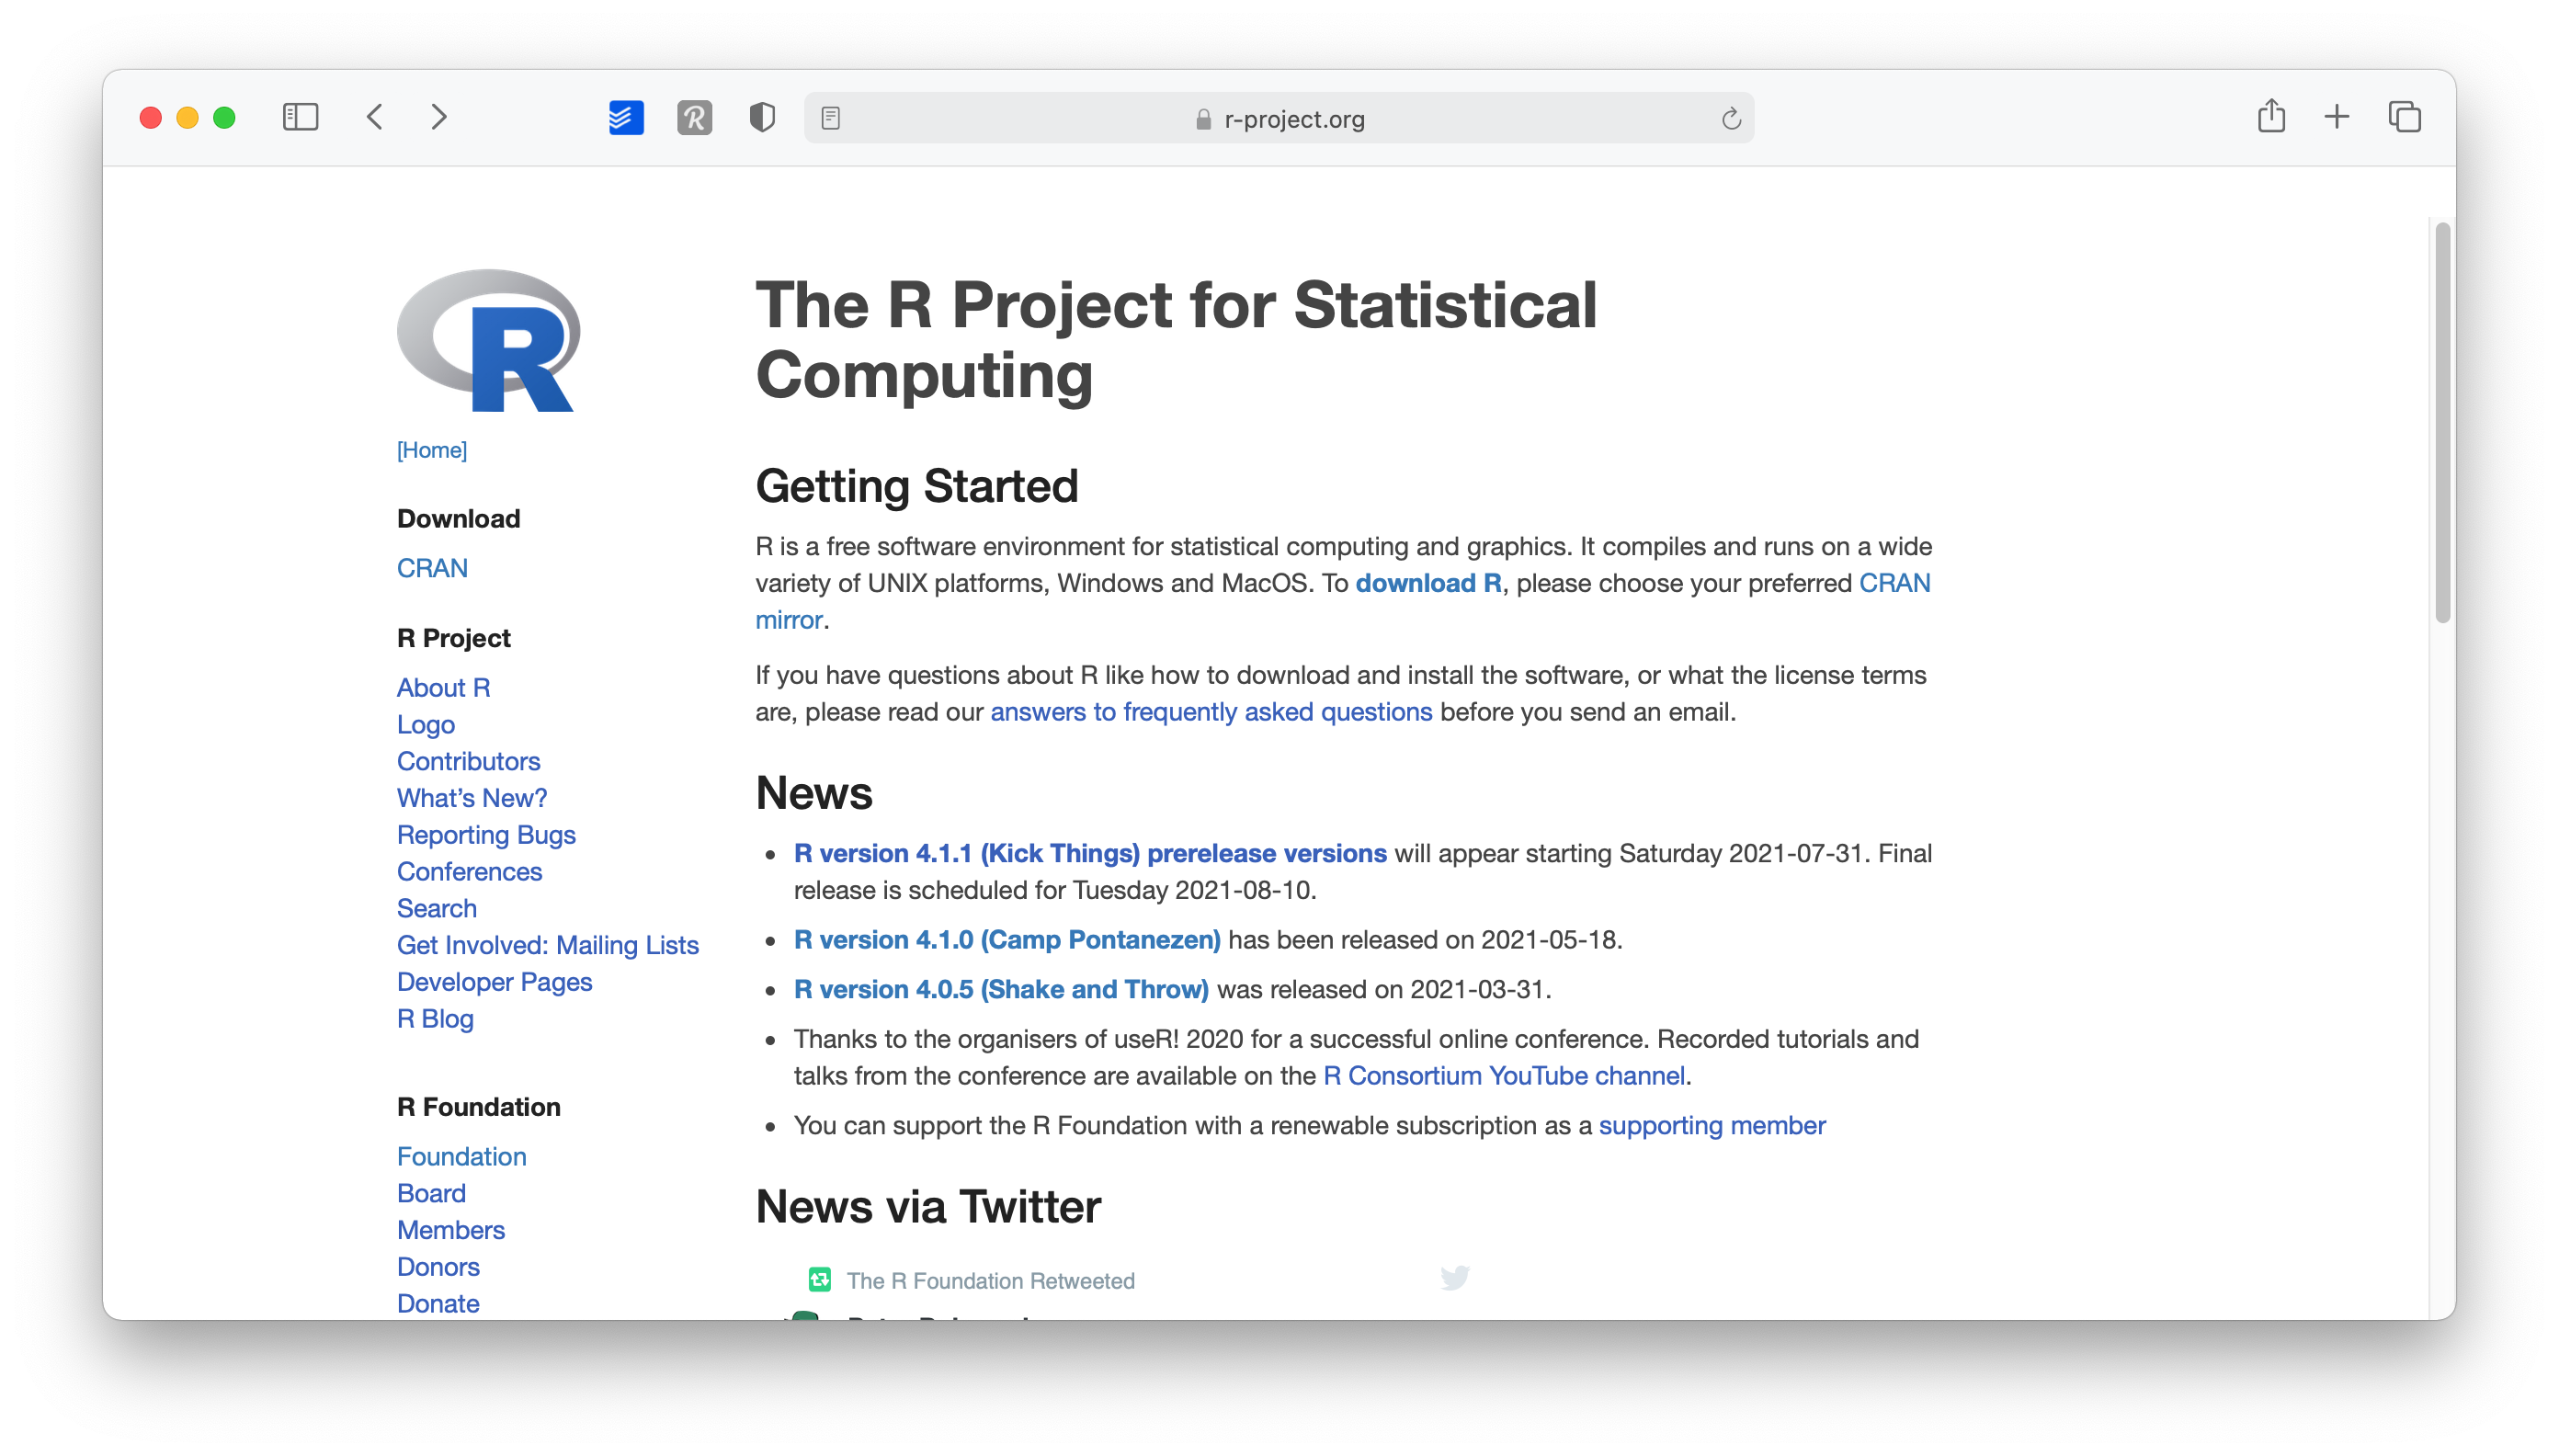
\includegraphics{images/chapter_03_img/r_project/00_r_project_page.png}
\item
  Click on \texttt{CRAN} where it says \texttt{Download}.
\item
  Choose a server in your country (all of them work, but downloads will
  perform quicker if you choose your country or one that is close to
  where you are).

  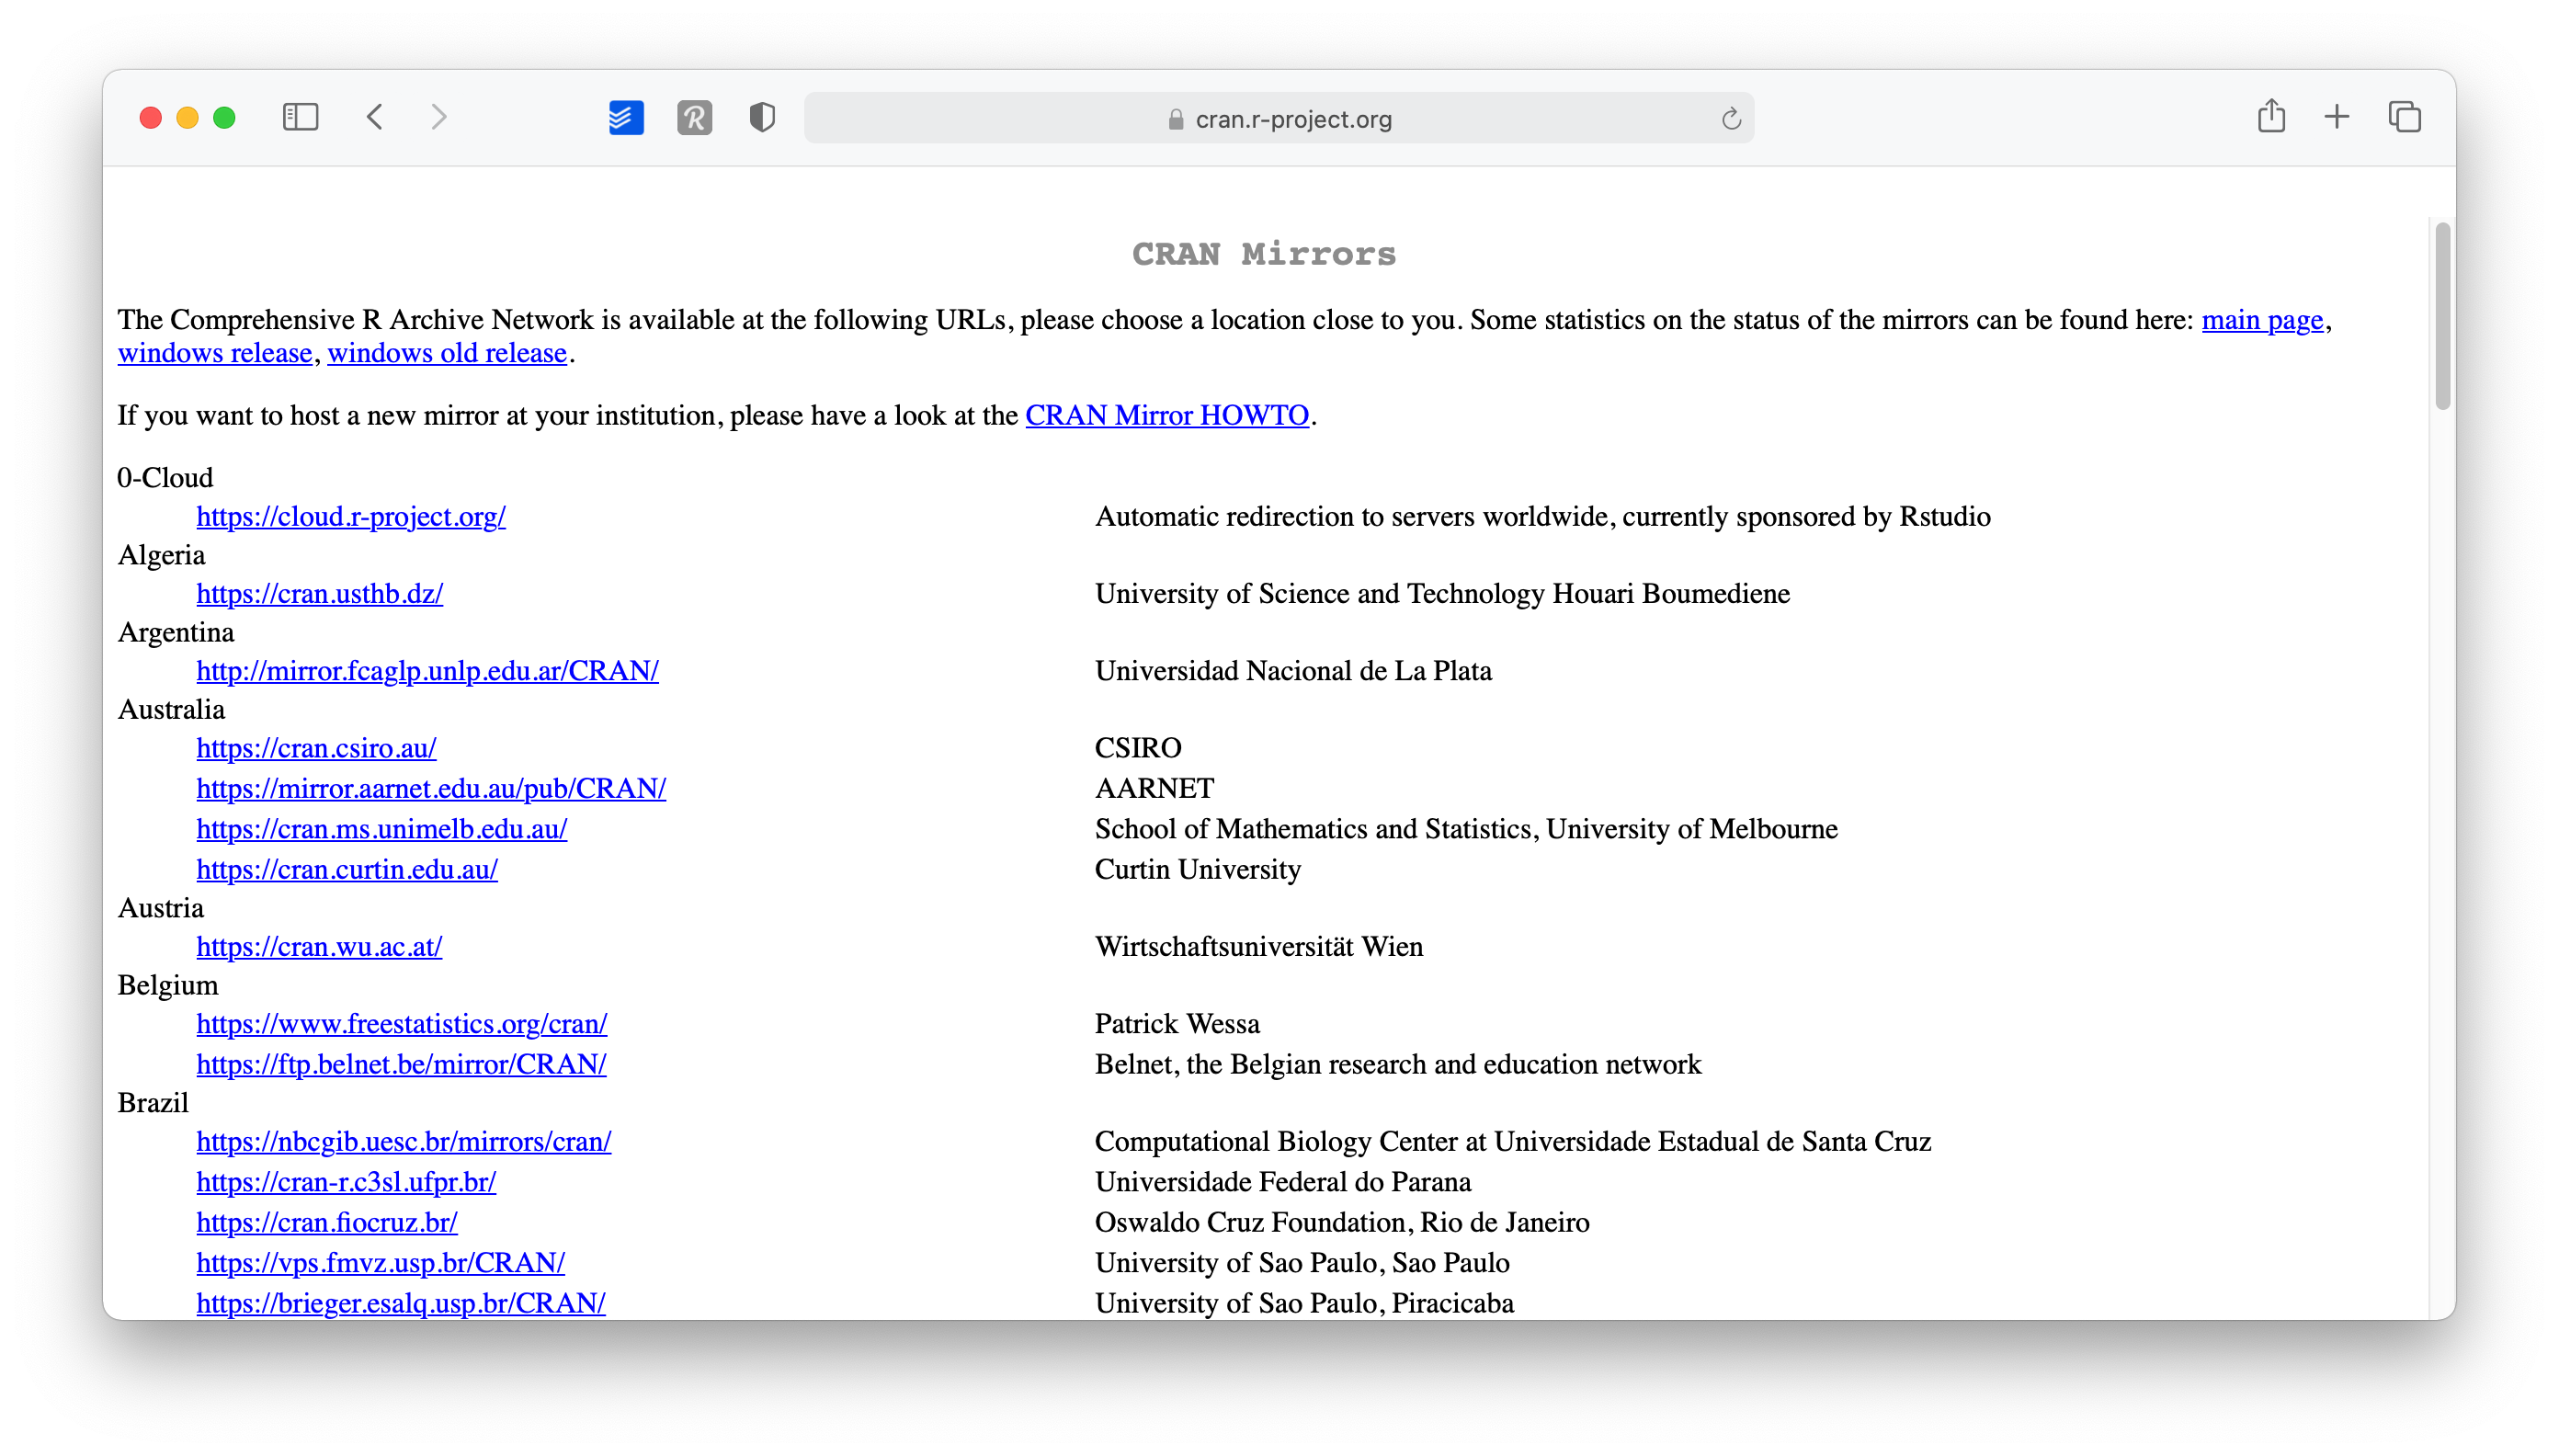
\includegraphics{images/chapter_03_img/r_project/01_r_project_cran_mirror.png}
\item
  Select the operating system for your computer, for example
  \texttt{Download\ R\ for\ macOS}.

  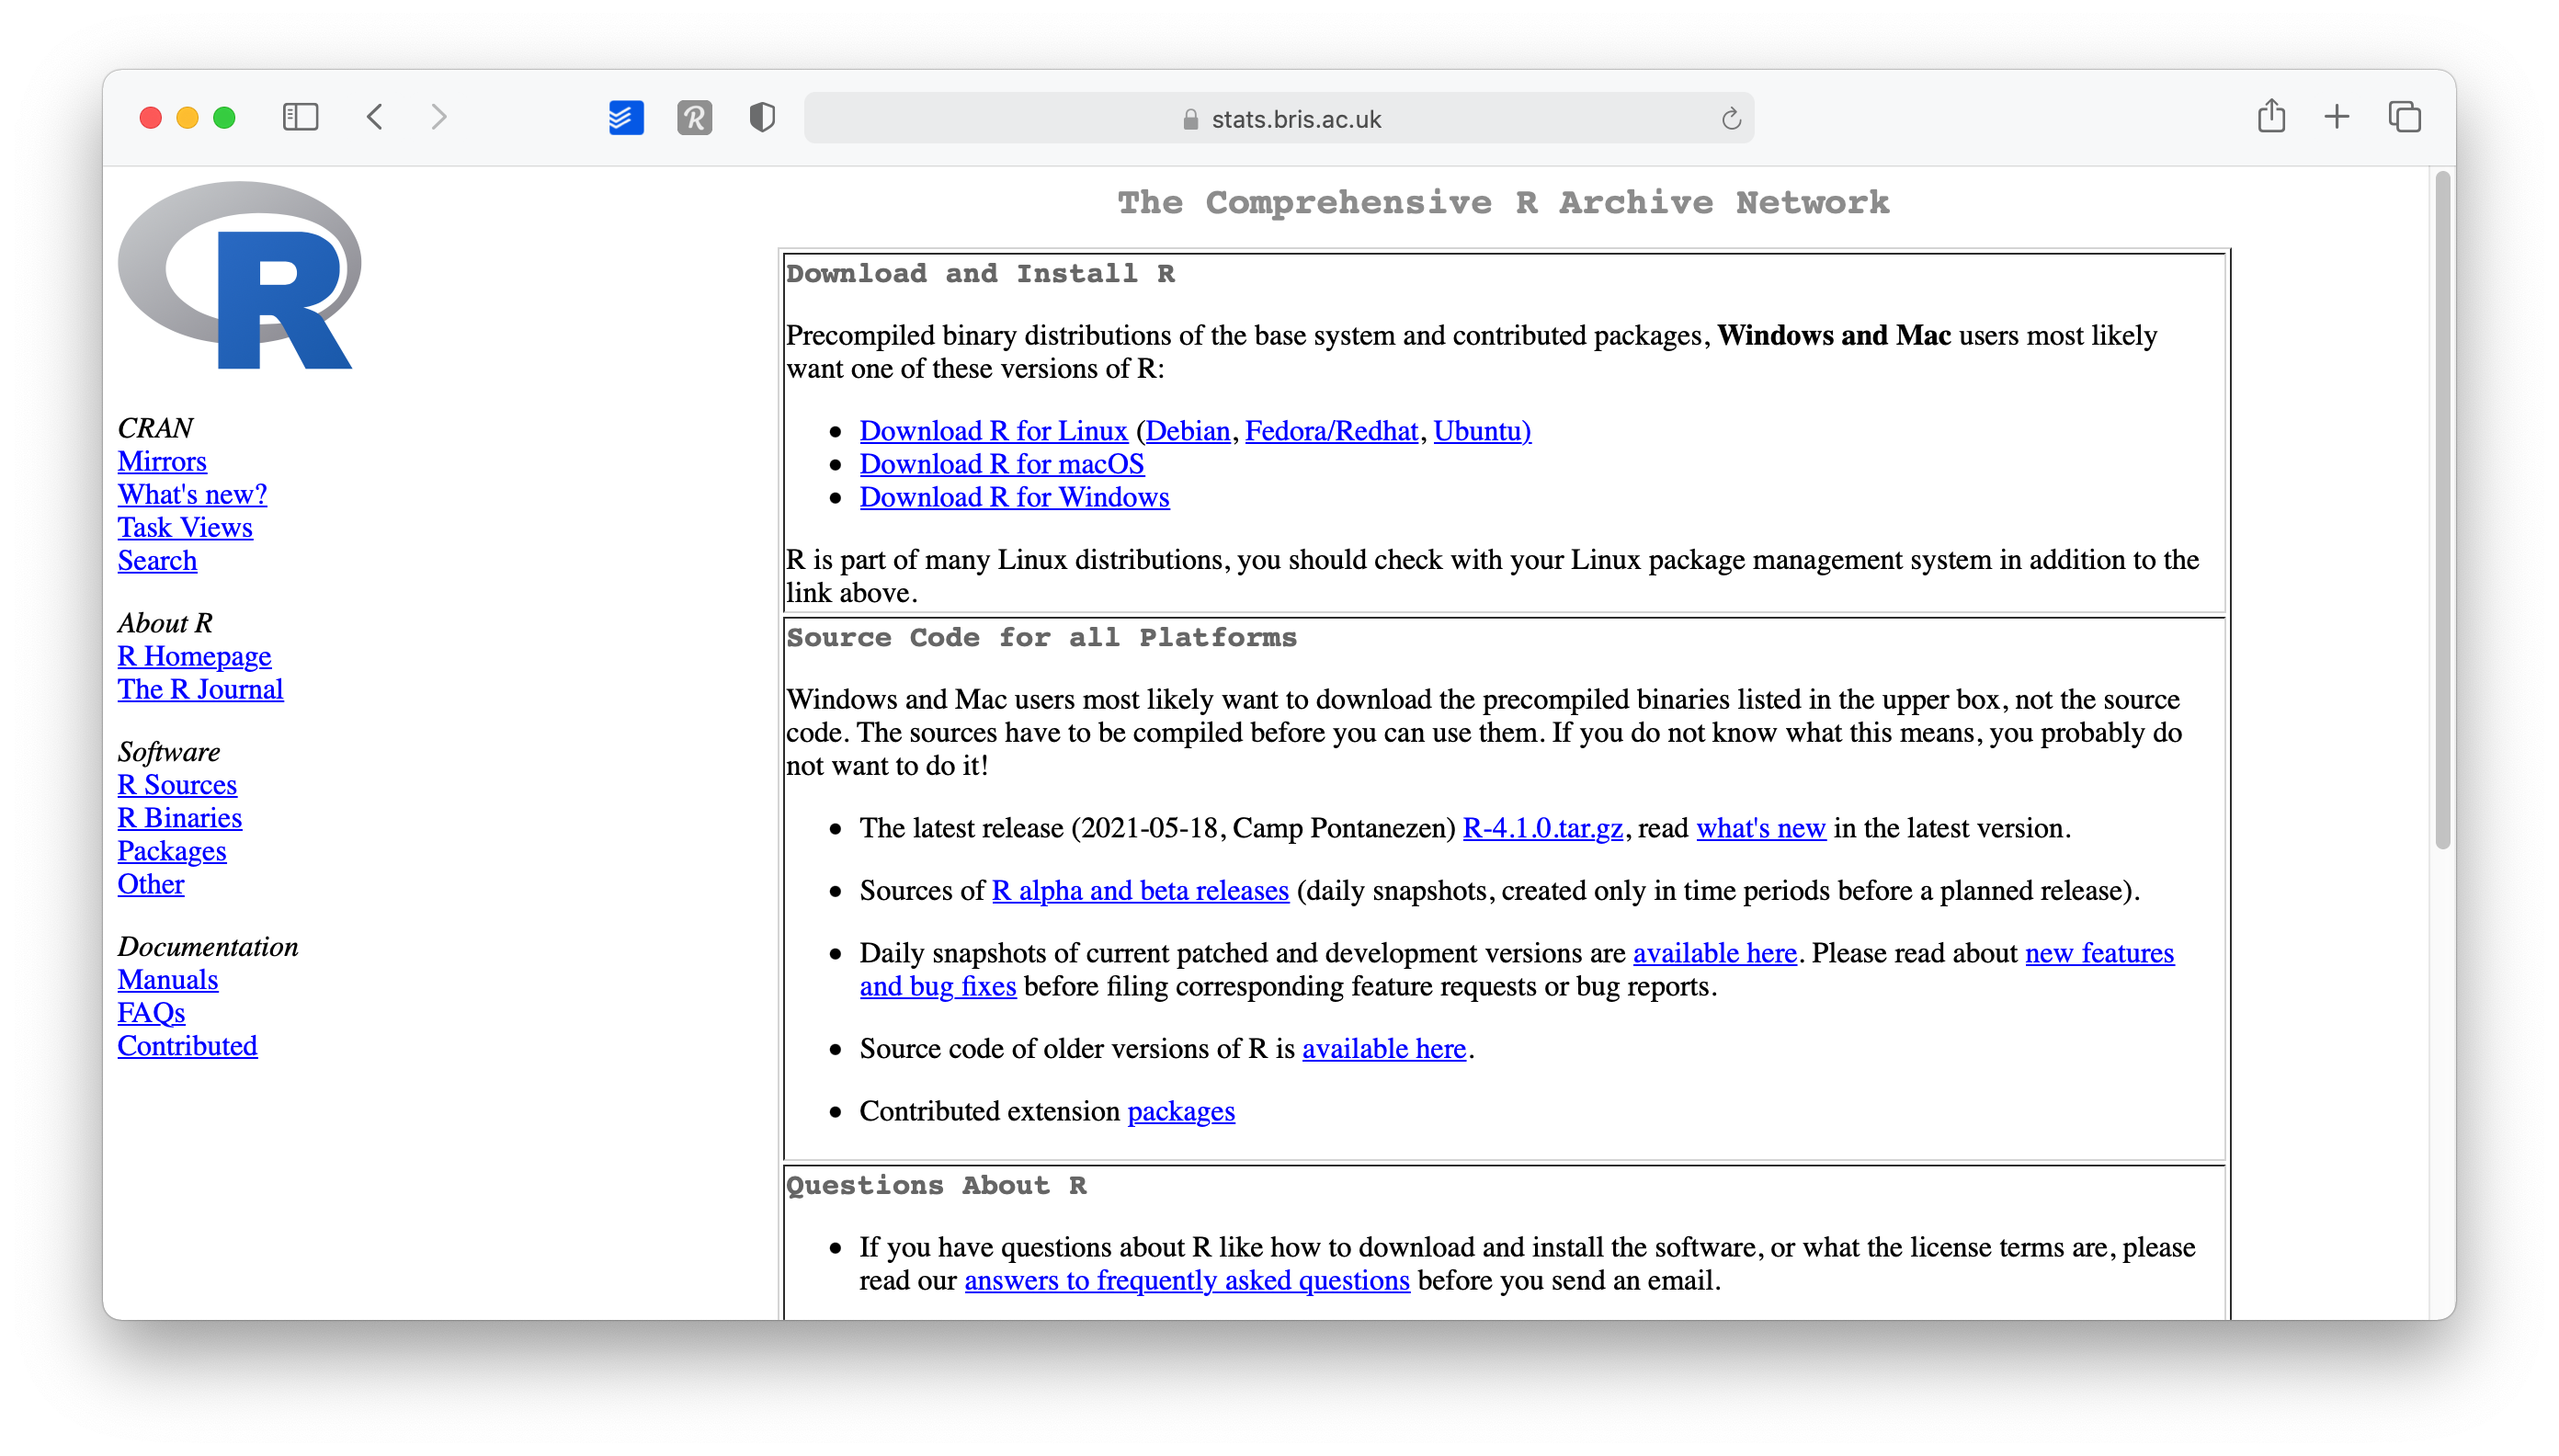
\includegraphics{images/chapter_03_img/r_project/02_r_project_os_choice.png}
\item
  Select the version you want to install (I recommend the latest
  version)

  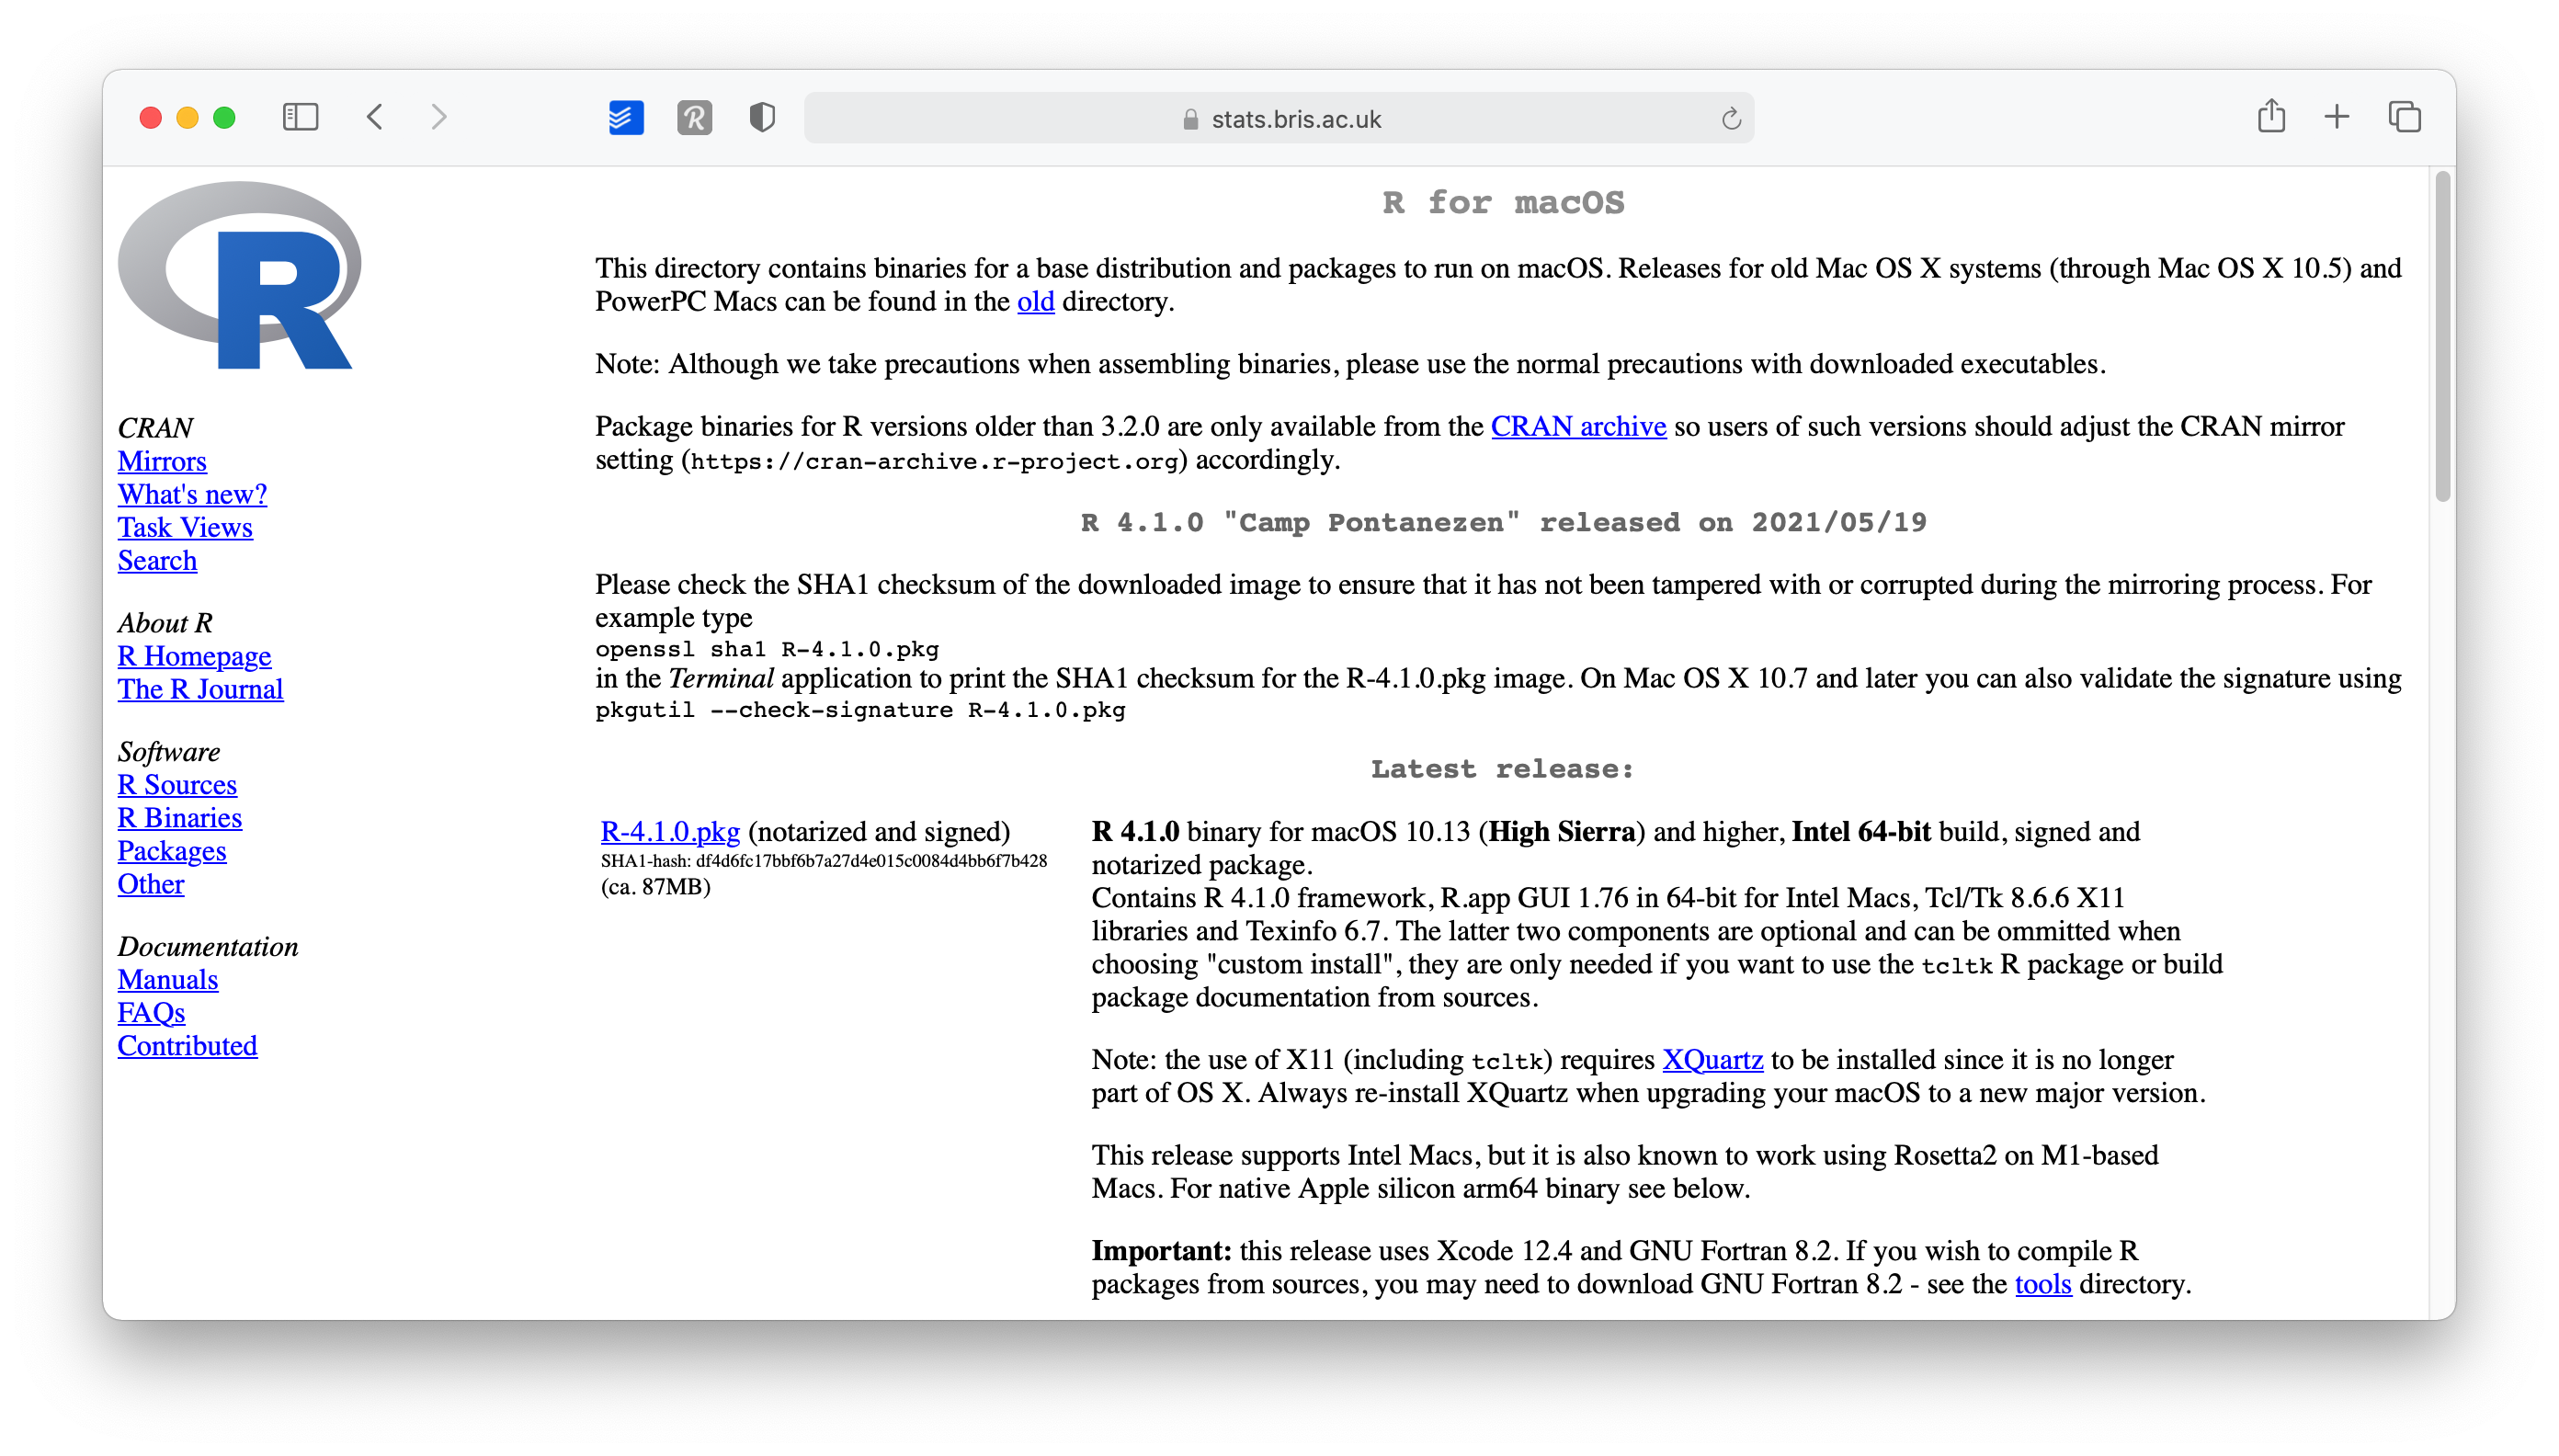
\includegraphics{images/chapter_03_img/r_project/03_r_project_version_choice.png}
\item
  Open the downloaded file and follow the installation instructions. I
  recommend leaving the suggested settings as they are.
\end{enumerate}

This was relatively easy. You now have \emph{R} installed. Technically
you can start using \emph{R} for your research, but there is one more
tool I strongly advise installing: RStudio.

\bookmarksetup{startatroot}

\chapter{The RStudio Interface}\label{the-rstudio-interface}

The RStudio interface is composed of quadrants, each of which fulfils a
unique purpose:

\begin{itemize}
\item
  The \texttt{Console} window,
\item
  The \texttt{Source} window,
\item
  The \texttt{Environment\ /\ History\ /\ Connections\ /\ Tutorial}
  window, and
\item
  The \texttt{Files\ /\ Plots\ /\ Packages\ /\ Help\ /\ Viewer} window
\end{itemize}

Sometimes you might only see three windows and wonder where the
\texttt{Source} window has gone in your version of RStudio. In order to
use it you have to either open a file or create a new one. You can
create a new file by selecting
\texttt{File\ \textgreater{}\ New\ File\ \textgreater{}\ R\ Script} in
the menu bar, or use the keyboard shortcut \texttt{Ctrl\ +\ Shift\ +\ N}
on PC and \texttt{Cmd\ +\ Shift\ +\ N} on Mac.

I will briefly explain the purpose of each window/pane and how they are
relevant to your work in \emph{R}.

\bookmarksetup{startatroot}

\chapter{\texorpdfstring{\emph{R} Basics: The very
fundamentals}{R Basics: The very fundamentals}}\label{r-basics-the-very-fundamentals}

After a likely tedious installation of \emph{R} and RStudio, as well as
a somewhat detailed introduction to the RStudio interface, you are
finally ready to \emph{`do'} things. By \emph{`doing'}, I mean
\emph{`coding'}. The term \emph{`coding'} in itself can instil fear in
some of you, but you only need one skill to do it: Writing. As mentioned
earlier, learning coding or programming means learning a new language.
However, once you have the basic grammar down, you already can
communicate quite a bit. In this section, we will explore the
fundamentals of \emph{R}. These build the foundation for everything that
follows. After that, we dive right into some analysis.

\section{\texorpdfstring{Basic computations in
\emph{R}}{Basic computations in R}}\label{basic-computations-in-r}

The most basic computation you can do in \emph{R} is arithmetic
operations. In other words, addition, subtraction, multiplication,
division, exponentiation and extraction of roots. In short, \emph{R} can
be used like your pocket calculator, or more likely the one you have on
your phone. For example, in Chapter @ref(the-console-window) we already
performed an addition. Thus, it might not come as a surprise how their
equivalents work in \emph{R}. Let's take a look at the following
examples:

\begin{Shaded}
\begin{Highlighting}[]
\CommentTok{\# Addition}
\DecValTok{10} \SpecialCharTok{+} \DecValTok{5}
\end{Highlighting}
\end{Shaded}

\begin{verbatim}
[1] 15
\end{verbatim}

\bookmarksetup{startatroot}

\chapter{\texorpdfstring{Starting your \emph{R}
projects}{Starting your R projects}}\label{starting-your-r-projects}

Every new project likely fills you with enthusiasm and excitement. And
it should. You are about to find answers to your research questions, and
you hopefully come out more knowledgeable due to it. However, there are
likely certain aspects of data analysis that you find less enjoyable. I
can think of two:

\begin{itemize}
\item
  Keeping track of all the files my project generates
\item
  Data wrangling
\end{itemize}

While we cover data wrangling in great detail in the next Chapter
(Chapter @ref(data-wrangling)), I would like to share some insights from
my work that helped me stay organised and, consequently, less
frustrated. The following applies to small and large research projects,
which makes it very convenient no matter the situation and the scale of
the project. Of course, feel free to tweak my approach to whatever suits
you. However, consistency is king.

\bookmarksetup{startatroot}

\chapter{Data Wrangling}\label{data-wrangling}

\begin{quote}
\textbf{Data wrangling} --- also called~\textbf{data
cleaning},~\textbf{data remediation}, or~\textbf{data munging}---refers
to a variety of processes designed to transform raw data into more
readily used formats. The exact methods differ from project to project
depending on the data you're leveraging and the goal you're trying to
achieve. (Stobierski 2021)
\end{quote}

You collected your data over months (and sometimes years), and all you
want to know is whether your data makes sense and reveals something
nobody would have ever expected. However, before we can truly go ahead
with our analysis, it is essential to understand whether our data is
`tidy'. What I mean is that our data is at the quality we would expect
it to be and can be reliably used for data analysis. After all, the
results of our research are only as good as our data and the methods we
deploy to achieve the desired insights.

\bookmarksetup{startatroot}

\chapter{Descriptive Statistics}\label{descriptive-statistics}

The best way to understand how participants in your study have responded
to various questions or experimental treatments is to use
\emph{descriptive statistics}. As the name indicates, their main purpose
is to `describe'. Most of the time, we want to describe the composition
of our sample and how the majority (or minority) of participants
performed.

In contrast, we use \emph{inferential statistics} to make predictions.
In Social Sciences, we are often interested in predicting how people
will behave in certain situations and scenarios. We aim to develop
models that help us navigate the complexity of social interactions that
we all engage in but might not fully understand. We cover
\emph{inferential statistics} in later chapters of this book.

In short, descriptive statistics are an essential component to
understand your data. To some extent, one could argue that we were
already describing our data when we performed various data wrangling
tasks (see Chapter @ref(data-wrangling)). The following chapters focus
on essential descriptive statistics, i.e.~those you likely want to
investigate in 99.9 out of 100 research projects.

This book takes a `visualised' approach to data analysis. Therefore,
each section will entail data visualisations and statistical computing.
A key learning outcome of this chapter is to plot your data using the
package \texttt{ggplot2} and present your data's characteristics in
different ways. Each chapter will ask questions about our dataset that
we aim to answer visually and computationally. However, first, we need
to understand how to create plots in \emph{R}.

\section{\texorpdfstring{Plotting in \emph{R} with
\texttt{ggplot2}}{Plotting in R with ggplot2}}\label{plotting-in-r-with-ggplot2}

Plotting can appear intimidating at first but is very easy and quick
once you understand the basics. The \texttt{ggplot2} package is a very
popular package to generate plots in \emph{R}, and many other packages
are built upon it. This makes it a very flexible tool to create almost
any data visualisation you could imagine. If you want to see what is
possible with \texttt{ggplot2}, you might want to consider looking at
\href{https://twitter.com/search?q=\%23tidytuesday}{\#tidytuesday} on
Twitter, where novices and veterans share their data visualisations
every week.

To generate any plot, we need to define three components at least:

\begin{itemize}
\item
  a dataset,
\item
  variables we want to plot, and
\item
  a function to indicate how we want to plot them, e.g.~as lines, bars,
  points, etc.
\end{itemize}

Admittedly, this is a harsh oversimplification, but it will serve as a
helpful guide to get us started. The function \texttt{ggplot()} is the
one responsible for creating any type of data visualisation. The generic
structure of a \texttt{ggplot()} looks like this:

\phantomsection\label{basic_ggplot_structure}
ggplot(data, aes(x = variable\_01, y = variable\_02))

In other words, we first need to provide the dataset \texttt{data}, and
then the aesthetics (\texttt{aes()}). Think of \texttt{aes()} as the
place where we define our variables (i.e.~\texttt{x} and \texttt{y}).
For example, we might be interested to know which movie genre is the
most popular among the top 250 IMDb movies. The dataset
\texttt{imdb\_top\_250} from the \texttt{r4np} package allows us to find
an answer to this question. Therefore we define the components of the
plot as follows:

\begin{itemize}
\item
  our data is \texttt{imdb\_top\_250}, and
\item
  our variable of interest is \texttt{genre\_01}.
\end{itemize}

\begin{Shaded}
\begin{Highlighting}[]
\FunctionTok{ggplot}\NormalTok{(imdb\_top\_250, }\FunctionTok{aes}\NormalTok{(}\AttributeTok{x =}\NormalTok{ genre\_01))}
\end{Highlighting}
\end{Shaded}

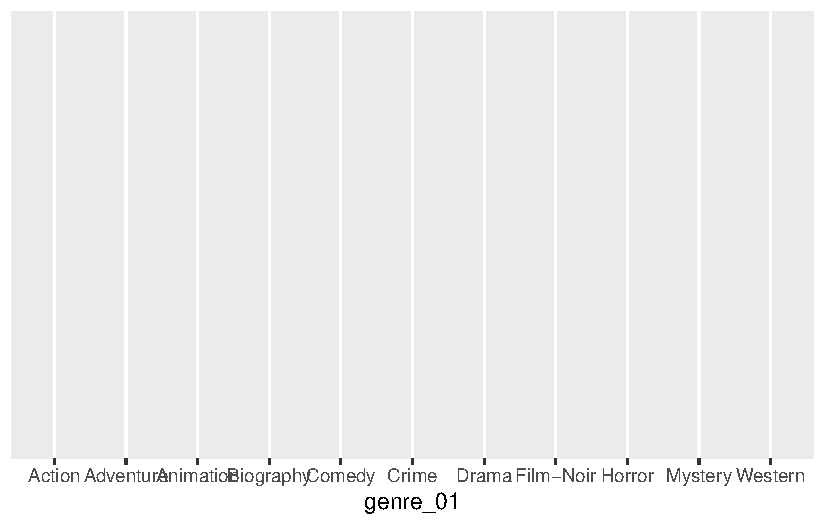
\includegraphics{08_descriptive_statistics_files/figure-pdf/most-popular-genre-incomplete-plot-1.pdf}

Running this line of code will produce an empty plot. We only get labels
for our x-axis since we defined it already. However, we have yet to tell
\texttt{ggplot()} how we want to represent the data on this canvas. Your
choice for how you want to plot your data is usually informed by the
type of data you use and the statistics you want to represent. For
example, plotting the mean of a factor is not meaningful, e.g.~computing
the mean of movie genres. On the other hand, we can count how often
specific genres appear in our dataset. One way of representing a
factor's count (or frequency) is to use a bar plot. To add an element to
\texttt{ggplot()}, i.e.~bars, we use \texttt{+} and append the function
\texttt{geom\_bar()}, which draws bars. The \texttt{+} operator works
similar to \texttt{\%\textgreater{}\%} and allows to chain multiple
functions one after the other as part of a \texttt{ggplot()}.

\begin{Shaded}
\begin{Highlighting}[]
\FunctionTok{ggplot}\NormalTok{(imdb\_top\_250, }\FunctionTok{aes}\NormalTok{(}\AttributeTok{x =}\NormalTok{ genre\_01)) }\SpecialCharTok{+}
  \FunctionTok{geom\_bar}\NormalTok{()}
\end{Highlighting}
\end{Shaded}

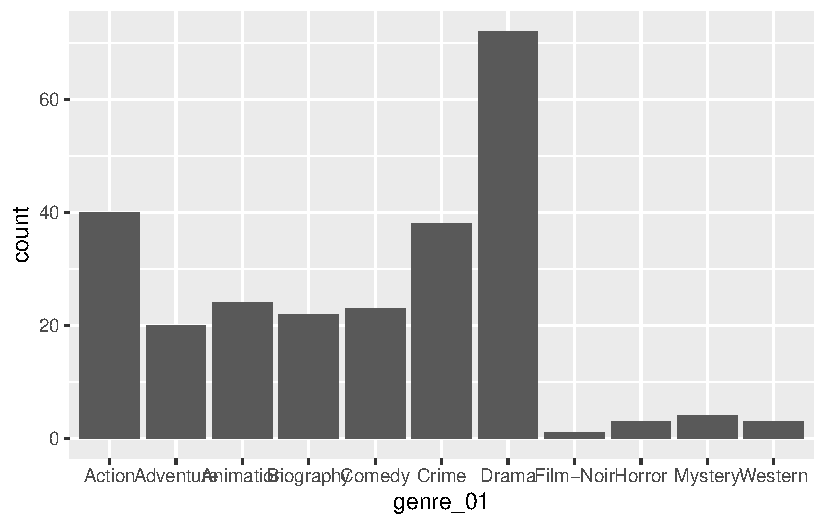
\includegraphics{08_descriptive_statistics_files/figure-pdf/most-popular-genre-with-barplot-1.pdf}

With only two lines of coding, we created a great looking plot. We can
see that \texttt{Drama} is by far the most popular genre, followed by
\texttt{Action} and \texttt{Crime}. Thus, we successfully found an
answer to our question. Still, there are more improvements necessary to
use it in a publication.

We can use \texttt{+} to add other elements to our plot, such as a title
and proper axes labels. Here are some common functions to further
customise our plot:

\begin{Shaded}
\begin{Highlighting}[]
\FunctionTok{ggplot}\NormalTok{(imdb\_top\_250, }\FunctionTok{aes}\NormalTok{(}\AttributeTok{x =}\NormalTok{ genre\_01)) }\SpecialCharTok{+}
  \FunctionTok{geom\_bar}\NormalTok{() }\SpecialCharTok{+}
  \FunctionTok{ggtitle}\NormalTok{(}\StringTok{"Most popular movie genres"}\NormalTok{) }\SpecialCharTok{+}  \CommentTok{\# Add a title}
  \FunctionTok{xlab}\NormalTok{(}\StringTok{"movie genre"}\NormalTok{) }\SpecialCharTok{+}                   \CommentTok{\# Rename x{-}axis}
  \FunctionTok{ylab}\NormalTok{(}\StringTok{"frequency"}\NormalTok{)                       }\CommentTok{\# Rename y{-}axis}
\end{Highlighting}
\end{Shaded}

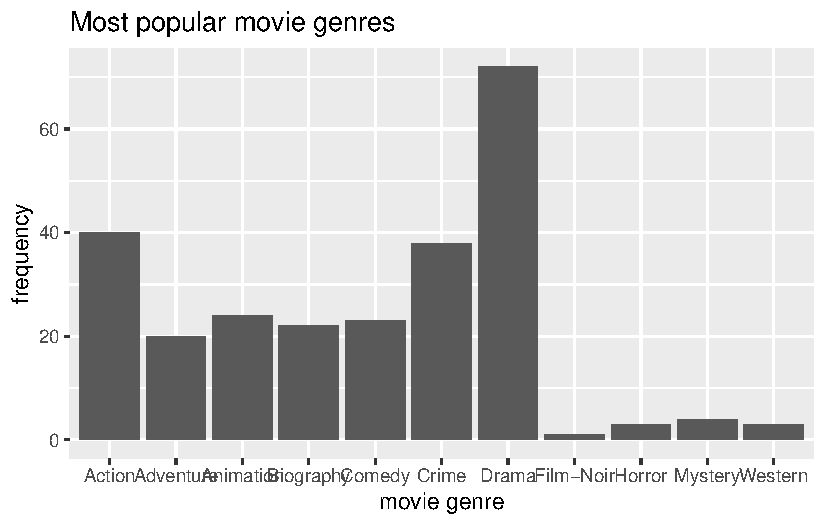
\includegraphics{08_descriptive_statistics_files/figure-pdf/most-popular-bar-plot-and-extras-1.pdf}

When working with factors, the category names can be rather long. In
this plot, we have lots of categories, and the labels
\texttt{Adventure}, \texttt{Animation}, and \texttt{Biography} are a bit
too close to each other for my taste. This might be an excellent
opportunity to use \texttt{coord\_flip()}, which rotates the entire plot
by 90 degrees, i.e.~turning the x-axis into the y-axis and vice versa.
This makes the labels much easier to read.

\begin{Shaded}
\begin{Highlighting}[]
\FunctionTok{ggplot}\NormalTok{(imdb\_top\_250, }\FunctionTok{aes}\NormalTok{(}\AttributeTok{x =}\NormalTok{ genre\_01)) }\SpecialCharTok{+}
  \FunctionTok{geom\_bar}\NormalTok{() }\SpecialCharTok{+}
  \FunctionTok{ggtitle}\NormalTok{(}\StringTok{"Most popular movie genres"}\NormalTok{) }\SpecialCharTok{+}
  \FunctionTok{xlab}\NormalTok{(}\StringTok{"movie genre"}\NormalTok{) }\SpecialCharTok{+}
  \FunctionTok{ylab}\NormalTok{(}\StringTok{"frequency"}\NormalTok{) }\SpecialCharTok{+}
  \FunctionTok{coord\_flip}\NormalTok{()}
\end{Highlighting}
\end{Shaded}

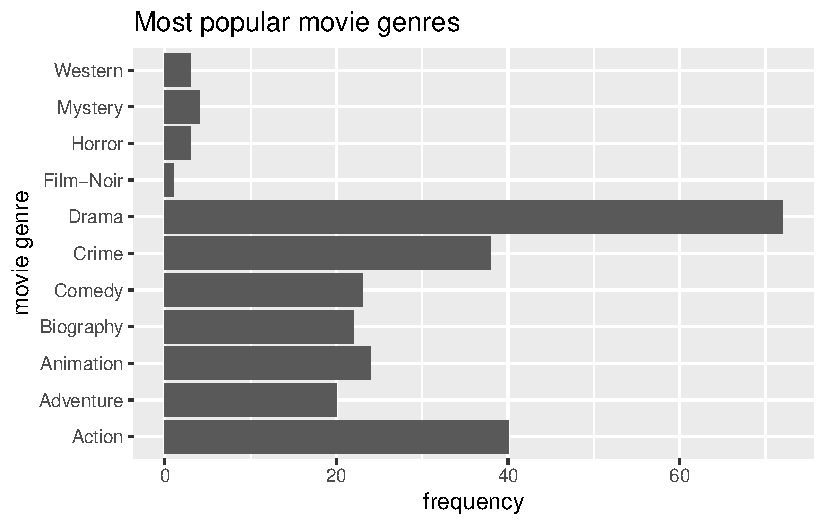
\includegraphics{08_descriptive_statistics_files/figure-pdf/popular-genre-barplot-extras-formatted-1.pdf}

Our plot is almost perfect, but we should take one more step to make
reading and understanding this plot even easier. At the moment, the bars
are ordered alphabetically by movie genre. Unfortunately, this is hardly
ever a useful way to order your data. Instead, we might want to sort the
data by frequency, showing the most popular genre at the top. To achieve
this, we could either sort the movies by hand (see Chapter
@ref(reordering-factor-levels)) or slightly amend what we have coded so
far.

The problem you encounter when rearranging a \texttt{geom\_bar()} with
only one variable is that we do not have an explicit value to indicate
how we want to sort the bars. Our current code is based on the fact that
\texttt{ggplot} does the counting for us. So, instead, we need to do two
things:

\begin{itemize}
\item
  create a table with all genres and their frequency, and
\item
  use this table to plot the genres by the frequency we computed
\end{itemize}

\begin{Shaded}
\begin{Highlighting}[]
\CommentTok{\# Step 1: The frequency table only}
\NormalTok{imdb\_top\_250 }\SpecialCharTok{\%\textgreater{}\%}
  \FunctionTok{count}\NormalTok{(genre\_01)}
\end{Highlighting}
\end{Shaded}

\begin{verbatim}
# A tibble: 11 x 2
   genre_01      n
   <fct>     <int>
 1 Action       40
 2 Adventure    20
 3 Animation    24
 4 Biography    22
 5 Comedy       23
 6 Crime        38
 7 Drama        72
 8 Film-Noir     1
 9 Horror        3
10 Mystery       4
11 Western       3
\end{verbatim}

\begin{Shaded}
\begin{Highlighting}[]
\CommentTok{\# Step 2: Plotting a barplot based on the frequency table}
\NormalTok{imdb\_top\_250 }\SpecialCharTok{\%\textgreater{}\%}
  \FunctionTok{count}\NormalTok{(genre\_01) }\SpecialCharTok{\%\textgreater{}\%}
  \FunctionTok{ggplot}\NormalTok{(}\FunctionTok{aes}\NormalTok{(}\AttributeTok{x =}\NormalTok{ genre\_01, }\AttributeTok{y =}\NormalTok{ n)) }\SpecialCharTok{+}

  \CommentTok{\# Use geom\_col() instead of geom\_bar()}
  \FunctionTok{geom\_col}\NormalTok{() }\SpecialCharTok{+}
  
  \CommentTok{\# Add titles for plot}
  \FunctionTok{ggtitle}\NormalTok{(}\StringTok{"Most popular movie genres"}\NormalTok{) }\SpecialCharTok{+}
  \FunctionTok{xlab}\NormalTok{(}\StringTok{"movie genre"}\NormalTok{) }\SpecialCharTok{+}
  \FunctionTok{ylab}\NormalTok{(}\StringTok{"frequency"}\NormalTok{) }\SpecialCharTok{+}
  
  \CommentTok{\# Rotate plot by 180 degrees}
  \FunctionTok{coord\_flip}\NormalTok{()}
\end{Highlighting}
\end{Shaded}

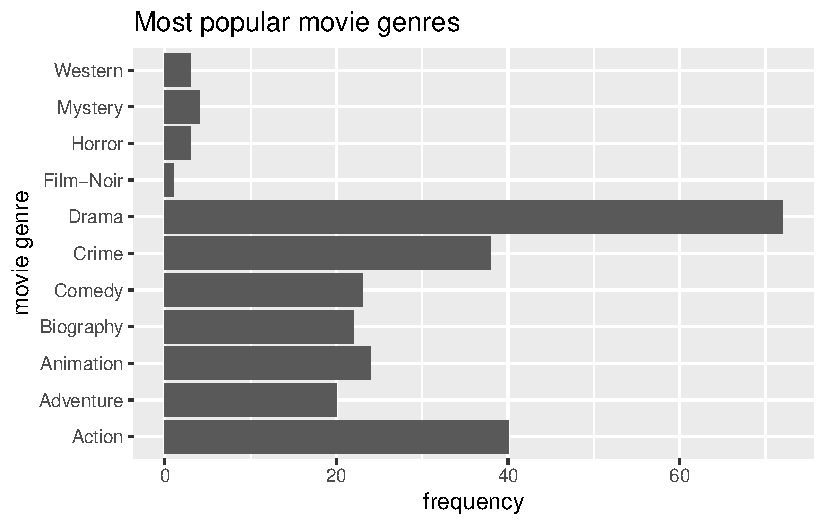
\includegraphics{08_descriptive_statistics_files/figure-pdf/unnamed-chunk-7-1.pdf}

\begin{Shaded}
\begin{Highlighting}[]
\CommentTok{\#Step 3: reorder() genre\_01 by frequency, i.e. by \textquotesingle{}n\textquotesingle{}}
\NormalTok{imdb\_top\_250 }\SpecialCharTok{\%\textgreater{}\%}
  \FunctionTok{count}\NormalTok{(genre\_01) }\SpecialCharTok{\%\textgreater{}\%}
  \FunctionTok{ggplot}\NormalTok{(}\FunctionTok{aes}\NormalTok{(}\AttributeTok{x =} \FunctionTok{reorder}\NormalTok{(genre\_01, n), }\AttributeTok{y =}\NormalTok{ n)) }\SpecialCharTok{+}  \CommentTok{\# Use \textquotesingle{}reorder()\textquotesingle{}}
  \FunctionTok{geom\_col}\NormalTok{() }\SpecialCharTok{+}
  \FunctionTok{ggtitle}\NormalTok{(}\StringTok{"Most popular movie genres"}\NormalTok{) }\SpecialCharTok{+}
  \FunctionTok{xlab}\NormalTok{(}\StringTok{"movie genre"}\NormalTok{) }\SpecialCharTok{+}
  \FunctionTok{ylab}\NormalTok{(}\StringTok{"frequency"}\NormalTok{) }\SpecialCharTok{+}
  \FunctionTok{coord\_flip}\NormalTok{()}
\end{Highlighting}
\end{Shaded}

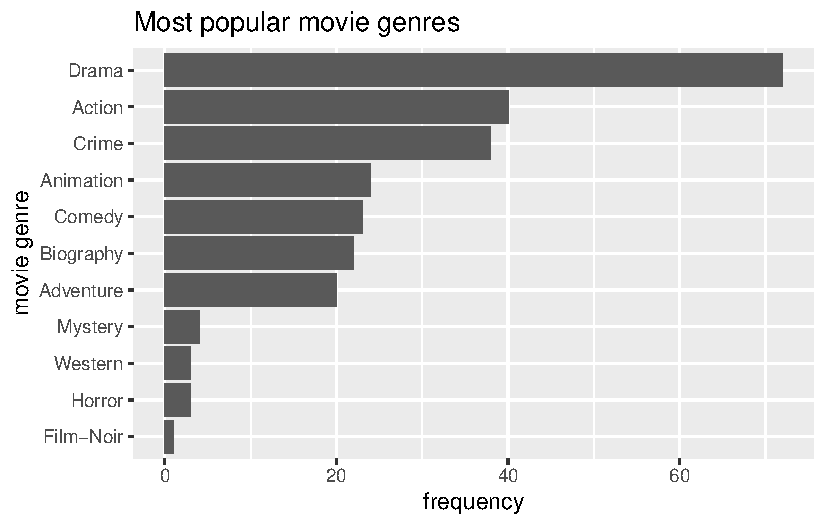
\includegraphics{08_descriptive_statistics_files/figure-pdf/unnamed-chunk-8-1.pdf}

Step 3 is the only code you need to create the desired plot. The other
two steps only demonstrate how one can slowly build this plot,
step-by-step. You might have noticed that I used \texttt{dplyr} to chain
all these functions together (i.e.~\texttt{\%\textgreater{}\%}), and
therefore, it was not necessary to specify the dataset in
\texttt{ggplot()}.

\bookmarksetup{startatroot}

\chapter{Sources of bias: Outliers, normality and other
`conundrums'}\label{sources-of-bias}

'\emph{Bias'} in your analysis is hardly ever a good thing unless you
are a qualitative researcher. Whether you consider it positive or
negative, we have to be aware of issues preventing us from performing a
specific type of analysis. All of the statistical computations discussed
in the following chapters can easily be affected by different sources of
bias. The lack of certain biases can be an assumption of particular
statistical tests. Thus, violating these assumptions would imply that
the analytical technique we use will produce wrong results, i.e.~biased
results. Field (2013) summarises three main assumptions we have to
consider:

\begin{itemize}
\item
  Linearity and additivity,
\item
  Independence,
\item
  Normality, and
\item
  Homogeneity of variance, i.e.~homoscedasticity.
\end{itemize}

\bookmarksetup{startatroot}

\chapter{Correlations}\label{correlations}

Sometimes counting and measuring means, medians, and standard deviations
is not enough because they are all based on a single variable. Instead,
we might have questions related to the relationship of two or more
variables. In this section, we will explore how correlations can (and
kind of cannot - see Chapter @ref(simpsons-paradox)) provide insights
into the following questions:

\begin{itemize}
\item
  Do movie viewers agree with movie critics regarding the rating of
  movies?
\item
  Do popular movies receive more votes from users than less popular
  movies?
\item
  Do movies with more votes also make more money?
\end{itemize}

\bookmarksetup{startatroot}

\chapter{Power: You either have it or you don't}\label{power-analysis}

The most frequently asked question by my students is: How much data do I
have to collect? My answer is always the same: \emph{`It depends'}. From
a student's perspective, this must be one of the most frustrating
answers. Usually, I follow this sentence up with something more helpful
to guide students on their way. For example, there is a way to determine
how large your sample has to be to detect specific relationships
reliably. This procedure is called \emph{power analysis}.

While \emph{power analysis} can be performed before and after data
collection, it seems rather pointless to do it afterwards when
collecting more data is not only challenging but sometimes impossible.
Thus, my explanations in this chapter will primarily focus on the
question: How much data is enough to detect relationships between
variables reliably.

\bookmarksetup{startatroot}

\chapter{Comparing groups}\label{comparing-groups}

Social Sciences is about the study of human beings and their
interactions. As such, we frequently want to compare two or more groups
of human beings, organisations, teams, countries, etc., with each other
to see whether they are similar or different from each other. Sometimes
we also want to track individuals over time and see how they may have
changed in some way or other. In short, comparing groups is an essential
technique to make inferences and helps us better understand the
diversity surrounding us.

If we want to perform a group comparison, we have to consider which
technique is most appropriate for our data. For example, some of it
might be related to the type of data we have collected, and other
aspects might be linked to the distribution of the data. More
specifically, before we apply any statistical technique, we have to
consider at least the following:

\bookmarksetup{startatroot}

\chapter{Regression: Creating models to predict future
observations}\label{regression}

Regressions are an exciting area of data analysis since it enables us to
make very specific predictions, incorporating different variables
simultaneously. As the name implies, regressions `regress', i.e., draw
on past observations to make predictions about future observations.
Thus, any analysis incorporating a regression makes the implicit
assumption that the past best explains the future.

I once heard someone refer to regressions as driving a car by looking at
the rear-view mirror. As long as the road is straight, we will be able
to navigate the car successfully. However, if there is a sudden turn, we
might drive into the abyss. This makes it very clear when and how
regressions can be helpful. Regressions are also a machine learning
method, which falls under \emph{models with supervised learning}. If you
find machine learning fascinating, you might find the book
\emph{``Hands-on Machine Learning with R''} (Boehmke and Greenwell 2019)
very insightful and engaging.

\bookmarksetup{startatroot}

\chapter{\texorpdfstring{Mixed-methods research: Analysing qualitative
data in
\emph{R}}{Mixed-methods research: Analysing qualitative data in R}}\label{mixed-methods-research}

Conducting mixed-methods research is challenging for everyone. It
requires an understanding of different methods and data types and
particular knowledge in determining how one can mix different methods to
improve the insights compared to a single method approach. This chapter
looks at one possibility of conducting mixed-methods research in
\emph{R}. It is likely the most evident use of computational software
for qualitative data.

While I consider myself comfortable in qualitative and quantitative
research paradigms, this chapter could be somewhat uncomfortable if you
are used to only one or the other approach, i.e.~only quantitative or
only qualitative research. However, with advancements in big data
science, it is impossible to code, for example, two million tweets
qualitatively. Thus, the presented methodologies should not be
considered in isolation from other forms of analysis. For some, they
might serve as a screening tool to sift through large amounts of data
and find those nuggets of most significant interest that deserve more
in-depth analysis. For others, these tools constitute the primary
research design to allow to generalise to a larger population. In short:
the purpose of your research will dictate the approach.

\bookmarksetup{startatroot}

\chapter{\texorpdfstring{Where to go from here: The next steps in your
\emph{R}
journey}{Where to go from here: The next steps in your R journey}}\label{next-steps}

The first steps have been made, but we can certainly not claim we have
reached our destination on this journey. If anything, this book helped
us reach the first peak in a series of mountains, giving us an overview
of what else there is to explore. To provide some guidance on where to
go next, I collated some resources worth exploring as a natural
continuation to this book.

\section{\texorpdfstring{GitHub: A Gateway to even more ingenious
\emph{R}
packages}{GitHub: A Gateway to even more ingenious R packages}}\label{next-steps-github}

If you feel you want more \emph{R} or you are curious to know what other
\emph{R} packages can do to complement your analysis, then GitHub brings
an almost infinite amount of options for you. Besides the CRAN versions
of packages, you find development versions of \emph{R} packages on
Github. These usually incorporate the latest features but are not yet
available through CRAN. Having said that, if you write your next
publication, it might be best to work with packages that are released on
CRAN. These are the most stable versions. After all, you don't want the
software to fail on you and hinder you from making that world-changing
discovery.

Still, more and more \emph{R} packages are released every day that offer
the latest advancements in statistical computations and beyond. Methods
covered in Chapter @ref(mixed-methods-research) are a great example of
what has become possible with advanced programming languages. So if you
want to live at the bleeding edge of innovative research methods, then
look no further.

However, GitHub also serves another purpose: To back up your research
projects and work collaboratively with others. I strongly encourage you
to create your own GitHub account, even just to try it. RStudio has
built-in features for working with GitHub, making it easy to keep track
of your analysis and ensure regular backups. Nobody wants to clean up
their data over months and lose it because their cat just spilt the
freshly brewed Taiwanese High Mountain Oolong Tea over one's laptop. I
use GitHub for many different things, hosting my blog
(\href{http://thesocialsciencesofa.com}{The Social Science Sofa}),
research projects, and this book.

There is much more to say about GitHub that cannot be covered in this
book, but if you seek an introduction, you might find
\href{https://www.youtube.com/user/github}{GitHub's Youtube Channel} of
interest or their \href{https://docs.github.com/en}{`Get started'}
guide. Best of all, setting up and using your GitHub account is free.

\section{Books to read and expand your
knowledge}\label{next-steps-books}

There are undoubtedly many more books to read, explore and use. However,
my number one recommendation to follow up with this book is
\href{https://r4ds.had.co.nz}{`R for Data Science'}. It takes your
\emph{R} coding beyond the context of Social Sciences and introduces new
aspects, such as \emph{`custom functions'} and \emph{`looping'}. These
are two essential techniques if you, for example, have to fit a
regression model for +20 subsets of your data, create +100 plots to show
results for different countries, or need to create +1000 of
individualised reports for training participants. In short, these are
very powerful (and efficient) techniques you should learn sooner than
later but are less essential for a basic understanding of data analysis
in \emph{R} for the Social Sciences.

If you want to expand your repertoire regarding data visualisations, a
fantastic starting point represents
\href{https://ggplot2-book.org}{`ggplot2: Elegant Graphics for Data
Analysis'} and \href{https://clauswilke.com/dataviz/}{`Fundamentals of
Data Visualization'}. However, these days I am looking mostly for
inspiration and new packages that help me create unique, customised
plots for my presentations and publications. Therefore, looking at the
source code of plots you like (for example, on GitHub) is probably the
best way to learn about \texttt{ggplot2} and some new techniques of how
to achieve specific effects (see also Chapter @ref(next-steps-twitter)).

If you are a qualitative researcher, you might be more interested in
what else you can do with \emph{R} to systematically analyse large
amounts of textual data (as was shown in Chapter
@ref(mixed-methods-research)). I started with the excellent book
\href{https://www.tidytextmining.com}{`Text Mining with R: A Tidy
Approach'}, which introduces you in greater depth to sentiment analysis,
correlations, n-grams, and topic modelling. The lines of qualitative and
quantitative research become increasingly blurred. Thus, learning these
techniques will be essential moving forward and pushing the boundaries
of what is possible with textual data.

\emph{R} can do much more than just statistical computing and creating
pretty graphs. For example, you can write your papers with it, even if
you do not write a single line of code. From Chapter
@ref(r-markdown-and-r-notebooks), you might remember that I explained
that \emph{R} Markdown files are an alternative to writing R scripts.
Suppose you want to deepen your knowledge in this area and finally let
go of Microsoft Word, I encourage you to take a peek at the
\href{https://bookdown.org/yihui/rmarkdown-cookbook/}{`R Markdown
Cookbook'} for individual markdown files and
\href{https://bookdown.org/yihui/bookdown/}{`bookdown: Authoring Books
and Technical Documents with R Markdown'} for entire manuscripts,
e.g.~journal paper submissions or books. I almost entirely abandoned
Microsoft Word, even though it served me well for so many years -
thanks.

Lastly, I want to make you aware of another open source book that covers
\href{https://rstats.wtf}{What They Forgot to Teach you About R} by
Jennifer Bryan and Jim Hester. It is an excellent resource to get some
additional insights into how one should go about working in \emph{R} and
\emph{RStudio}.

\section{\texorpdfstring{Engage in regular online readings about
\emph{R}}{Engage in regular online readings about R}}\label{next-steps-online-readings}

A lot of helpful information for novice and expert \emph{R} users is not
captured in books but online blogs. There are several that I find
inspiring and an excellent learning platform, each focusing on different
aspects.

The most comprehensive hub for all things \emph{R} is undoubtedly
\href{https://www.r-bloggers.com}{`R-bloggers'}. It is a blog aggregator
which focuses on collecting content related to \emph{R}. I use it
regularly to read more about new packages, new techniques, helpful
tricks to become more `fluent' in \emph{R} or simply find inspiration
for my own \emph{R} packages. More than once, I found interesting blogs
by just reading posts on `R-bloggers'. For example, the day I wrote this
chapter, I learned about \texttt{emayili}, which allows you to write
your emails from \emph{R} using \emph{R} markdown. So not even the sky
is the limit, it seems.

Another blog worth considering is the one from
\href{https://www.tidyverse.org/blog/}{`Tidyverse'}. This blog is hosted
and run by RStudio and covers all packages within the
\texttt{tidyverse}. Posts like
\href{https://www.tidyverse.org/blog/2021/08/waldo-0-3-0/}{`waldo
0.3.0'} made my everyday data wrangling tasks a lot easier because
finding the differences between two datasets can be like searching a
needle in a haystack. For example, it is not unusual to receive two
datasets that contain the same measures, but some of their column names
are slightly different, which does not allow us to merge them in the way
we want quickly. I previously spent days comparing and arranging
multiple datasets with over 100 columns. Let me assure you, it is not
really fun to do.

The blog \href{https://www.data-imaginist.com}{`Data Imaginist'} by
Thomas Lin Pedersen covers various topics around data visualisations. He
is well known for his Generative Art, i.e.~art that is computationally
generated. But one of my favourite packages, \texttt{patchwork}, was
written by him and gained immense popularity. It has never been easier
to arrange multiple plots with such little code.

Lastly, I want to share with you the
\href{https://www.cedricscherer.com/top/dataviz/}{blog of Cédric
Scherer} for those of you who want to learn more about high-quality data
visualisations based on \texttt{ggplot2}. His website hosts many
visualisations with links to the source code on GitHub to recreate them
yourself. It certainly helped me improve the visual storytelling of my
research projects.

\section{Join the Twitter community and hone your
skills}\label{next-steps-twitter}

Learning \emph{R} means you also join a community of like-minded
programmers, researchers, hobbyists and enthusiasts. Whether you have a
Twitter account or not, I recommend looking at the
\href{https://twitter.com/search?q=\%23rstats}{\#RStats} community
there. Plenty of questions about \emph{R} programming are raised and
answered on Twitter. In addition, people like to share insights from
their projects, often with source code published on GitHub. Even if you
are not active on social media, it might be worth having a Twitter
account just to receive news about developments in \emph{R} programming.

As with any foreign language, if we do not use it regularly, we easily
forget it. Thus, I would like to encourage you to take part in
\href{https://www.tidytuesday.com}{Tidy Tuesday}. It is a weekly
community exercise around data visualisation and data wrangling. In
short: You download a dataset provided by the community, and you are
asked to create a visualisation as simple or complex as you wish. Even
if you only manage to participate once a month, it will make you more
`fluent' in writing your code. Besides, there is a lot to learn from
others because you are also asked to share the source code. This
activity takes place on Twitter, and you can find contributions by using
\href{https://twitter.com/search?q=\%23tidytuesday}{\#TidyTuesday}.
Whether you want to share your plots is up to you, but engaging with
this activity will already pay dividends. Besides, it is fun to work
with datasets that are not necessarily typical for your field.

\bookmarksetup{startatroot}

\chapter*{References}\label{references}
\addcontentsline{toc}{chapter}{References}

\markboth{References}{References}

\phantomsection\label{refs}
\begin{CSLReferences}{1}{0}
\bibitem[\citeproctext]{ref-boehmke2019hands}
Boehmke, Brad, and Brandon Greenwell. 2019. \emph{Hands-on Machine
Learning with r}. Chapman; Hall/CRC.

\bibitem[\citeproctext]{ref-field2013discovering}
Field, Andy. 2013. \emph{Discovering Statistics Using IBM SPSS
Statistics}. Sage Publications.

\bibitem[\citeproctext]{ref-hsbDataWrangling}
Stobierski, Tim. 2021. {``Data Wrangling: What It Is and Why It's
Important.''} Harvard Business School Online.
\url{https://online.hbs.edu/blog/post/data-wrangling}.

\end{CSLReferences}



\backmatter
\printindex

\end{document}
